\documentclass{beamer} % [aspectratio=169]
\usetheme{ucl}
\setbeamercolor{banner}{bg=darkred}
\setbeamersize{description width=2em}
\setbeamertemplate{navigation symbols}{\vspace{-2ex}} 

\usepackage[T1]{fontenc} % Turn £ into $
\usepackage{minted}
\usemintedstyle{emacs}

\usepackage{fancyvrb}
\usepackage{xcolor}
\usepackage{url}

\usepackage{natbib}
\usepackage{bibentry}
\usepackage{url}

\newenvironment{variableblock}[3]{%
  \setbeamercolor{block body}{#2}
  \setbeamercolor{block title}{#3}
  \begin{block}{#1}}{\end{block}}

\newcommand\emc[1]{\textcolor{midred}{\textbf{#1}}}

\AtBeginSection[]{
  \begin{frame}
  \vfill
  \centering
  \begin{beamercolorbox}[sep=8pt,center,shadow=true,rounded=true]{title}
    \usebeamerfont{title}\insertsectionhead\par%
  \end{beamercolorbox}
  \vfill
  \end{frame}
}

\author{Prof.\ Mark Handley \\ University College London, UK\\
\small{Based on slides from George Danezis}}
\title{Basics of Computer Programming \\ \& Software Engineering.}
\subtitle{ENGF0002: Design and Professional Skills }
% \institute{}
\date{Term 1, 2018}

\begin{document}
\nobibliography*

\frame{
\titlepage
}

\section{Introduction}

\frame{
\frametitle{Introducing Basics.}

In the `Basics' topic we will:
\begin{itemize}
\item Introduce basic Python \emc{language} concepts.
\item Illustrate \emc{algorithms}, to perform numerical computations.
\item Expose you to the problems of \emc{correctness}, and \emc{testing}.
\item Introduce \emc{good practices} when programming.
\end{itemize}

} 


\frame{
\frametitle{What is Computer Science \& Software Engineering?}

Computer Science:
\begin{itemize}
\item Studies the nature of \emc{information, computation, complexity} of algorithms, and their \emc{correctness}.
\item Deep mathematical foundations, including logic, algebra and probability theory.
\end{itemize}

Software Engineering:
\begin{itemize}
\item Studies how teams can repeatably \emc{build high quality, correct, usable and efficient software}, to meet \emc{people's needs}.
\item Programming is a foundational and important part of it.
\end{itemize}

The two are interlinked, and we will study them together.
} 

\frame{
\frametitle{Programming \& languages (I).}

Programming \& Programmability: 
\begin{itemize}
	\item A device is programmable if it allows a programmer (developer, engineer) to \emc{alter its behavior}. This is the act of programming.
	\item We usually think of a device as programmable, when the \emc{program itself takes the form or information}, rather than physical modification.
	\item A computer is the \emc{ultimate programmable device}, and can execute all computations. Simpler ones include video recording devices, microwave ovens, and alarm clocks.
	\item \emc{Programming is specializing} a device to solve \emc{a problem that people have}.
\end{itemize}
}

\frame{
\frametitle{Programming \& languages (II).}

Programming Languages:
\begin{itemize}
	\item The \emc{information describing the program} (code), is expressed in a programming language.
	\item \emc{Trivial} programming languages: button pressed to program an alarm clock. They are very \emc{low-level ways}, and lead to errors and inflexibility.
	\item Full computers are programmed in \emc{higher-level formal languages}. Programmers may express their intent directly, build complex abstractions, and compose programs from smaller fragments.
	\item Programming languages are formal languages but also \emc{human languages}. Programmers, use them to \emc{express and communicate their intent}.
\end{itemize}

}


\frame{
\frametitle{Why Python?} 
\begin{itemize}
	\item \emc{Real-world}, widely used programming language \\(4th in 2018 TIOBE ranking.)
	\item \emc{Multi-paradigm}: scripting, procedural, functional elements, object oriented, generics.
	\item Extensive \emc{eco-system} of tools and libraries. Great documentation.
	\item Significant \emc{industrial uses}.
	\item \emc{High-productivity}, and perfect for rapid prototyping.
\end{itemize}

\vspace{3mm}
A \emc{weakness} we will turn to a strenth:
\begin{itemize}
	\item It does not force you to adopt \emc{good programming practices}.
	\item It \emc{supports them}, but you must learn them!
\end{itemize}


}

\frame{
	
\frametitle{Other languages you might want to learn.}

\emc{Different problems} may require \emc{different tools}:
\begin{itemize}
\item Lower-level: Rust$*$, C++, \emc{C} --- COMP101P.
\item Static typing: Go$*$, \emc{Java}, C\# --- COMP103P.
\item Web: Javascript$*$.
\item Functional: \emc{Haskell}, Scala$*$ --- COMP101P.
\end{itemize}


\vspace{1mm}
$*$ - trendy languages at the moment

\vspace{3mm}
All programming languages mix and match a few principles. \\
Good computer scientists \emc{know those principles},\\ and can \emc{work in any language}.
}

\begin{frame}[fragile]
\frametitle{Using Python interactively.} 

\begin{itemize}
	\item Python 3.7. (\url{https://www.python.org/about/gettingstarted/})
	\item Open a command line console, and run the Python interpreter.
	\item Type your fist command: \mint{Python}{print("Hello World!")}
	\item You should see it executing!

\begin{Verbatim}[fontsize=\footnotesize]
mjh$ python3
Python 3.7.0 (default, Jun 28 2018, 05:55:06) 
[Clang 9.1.0 (clang-902.0.39.2)] on darwin
Type "help", "copyright", "credits" or "license" for more information.
>>> print("Hello World!")
Hello World!
>>> 
\end{Verbatim}

\end{itemize}

\end{frame}


\frame{
\frametitle{Key resources and tools.} 

The interactive interpreter is only good for quick experimentation.
\begin{itemize}
	\item \emc{Code editor}: atom (hip!), Sublime (hip!), Visual Studio Code. \\ Must haves: Good syntax highlighting, good handling of files \& folders, whitespace, looks very cool.
	\item \emc{Browser} with Python \emc{Documentation}: \url{https://docs.python.org/3/}. \\ (including Python \emc{tutorial} and \emc{Library reference}.)
	\item \emc{Command line} \& learn how to use it. \url{https://www.lynda.com/Linux-tutorials/Learn-Linux-Command-Line-Basics/435539-2.html}
	\item \emc{Stack Overflow} for Q\&A. \\ \url{https://stackoverflow.com/}
	\item \emc{Install pytest}. \url{https://docs.pytest.org/}
\end{itemize}
}

\frame{
\frametitle{Your physical \& mental well being.} 

\begin{itemize}
\item Approach the physical activity of programming with \emc{professionalism}.
\item Think of the \emc{ergonomics} of your physical environment: chair height, desk, posture, keyboard style, monitor type and positioning.
\item Make sure you \emc{enjoy your working environment}: light, sounds, distractions.
\item \emc{Take breaks}, at least every hour.
\end{itemize}

}

\begin{frame}[fragile]
\frametitle{The `Hello World!' program in Python.} 

Programs live in files. A simple Python program:

	\inputminted[
		xleftmargin=1.4em,
		frame=lines,
		framesep=2mm,
		%baselinestretch=1.2,
		bgcolor=stone,
		fontsize=\footnotesize,
		linenos
	]{python}{src/hello_world.py}

Execute your first program, by running:
\begin{Verbatim}
$ python3 hello_world.py
Hello World!
\end{Verbatim}

\end{frame}

\begin{frame}
\frametitle{Comments}

Comments are not executed by Python, but form part of your program.
\begin{itemize}
\item Comments \emc{communicate intent} to your future self and others.
\item Express in comments concepts you cannot directly express in code.
\item Prefer to express concepts directly in code.
\item Keep comments local to the relevant code.
\item Do not overcomment; avoid duplicate, redundant or wrong comments. 
\item Every comment will have to be maintained in the future.
\end{itemize}
\end{frame}

\begin{frame}
\frametitle{Whitespace.}

Python is \emc{sensitive to indentation} using whitespace. Use 3 or 4 spaces (not a tab) to indent blocks of code. More about this later \ldots.

	\inputminted[
		xleftmargin=1.4em,
		frame=lines,
		framesep=2mm,
		%baselinestretch=1.2,
		bgcolor=stone,
		fontsize=\footnotesize,
		linenos
	]{python}{src/hello_world.py}

\end{frame}

\begin{frame}
\frametitle{How do we know a program does what it should?}

\emc{Correctness is the most important problem} in software engineering and computer science!

\vspace{3mm}
\emc{Testing is the key technique} to produce high quality, correct programs. It is an activity that is continuous, and performed in parallel with programming.

\vspace{3mm}
Complimentary techniques for ensuring program correctness include \emc{formal verification}. Those are more expensive, but necessary to reason about very complex problems.

\vspace{3mm}
Finally, formal periodic \emc{code reviews}, or continuous reflection through \emc{pair programming} also improve quality.

\end{frame}


\frame{
\frametitle{Test Code Continuously.} 

\emc{Testing} is the most important technique to gain confidence a program does what it should:
\begin{itemize}
	\item Unit Test every 2-5 lines of code you write. Think how to \emc{test every snippet of code} just before, while, or just after you write it.
	\item Use a mature \emc{tool for testing} your programs. We will use \texttt{pytest}. \url{https://docs.pytest.org/}.
	\item \emc{Different testing techniques} for code correctness, integration, security, performance and user experience.
	\item Shortcomings of testing: \emc{lack of completeness}.
\end{itemize}

}

\frame{
\frametitle{Testing the `Hello World!' program.} 

\emc{Tests are snippets of code} executing parts of your program. \\ Eg.\ the test of the simple Python program is:

	\inputminted[
		xleftmargin=1.4em,
		frame=lines,
		framesep=2mm,
		%baselinestretch=1.2,
		bgcolor=stone,
		fontsize=\footnotesize,
		linenos
	]{python}{src/test_hello_world.py}

We run the \emc{test suite}, by executing \texttt{pytest test\_hello\_world.py} on the command line.


}

\frame{
\frametitle{Code documentation and its tests. } 

\emc{Code documentation} is not executed, but forms part of the program. It is useful to your future self, or others that want to use part of your program. Hence, \emc{document reusable units of code}.

	\inputminted[
		xleftmargin=1.4em,
		highlightlines={6-7},
		frame=lines,
		framesep=2mm,
		%baselinestretch=1.2,
		bgcolor=stone,
		fontsize=\footnotesize, 
		linenos
	]{python}{src/hello_world_doc.py}

You must \emc{test code in documentation}. \\ \texttt{pytest -vs --doctest-modules test\_hello\_world.py}.

}


\begin{frame}[fragile]

\frametitle{Example of a successful test run. }

Executing \texttt{pytest} runs all tests in functions named \texttt{test\_*} and documentation strings.

\begin{Verbatim}[fontsize=\scriptsize]
$ pytest -vs --doctest-modules src/*hello*.py
=================================== test session starts ====================================
platform darwin -- Python 3.7.0, pytest-3.7.4, py-1.6.0, pluggy-0.7.1 -- /opt/local/Library/Frameworks/Python.framework/Versions/3.7/bin/python3.7
cachedir: .pytest_cache
rootdir: /Users/mjh/teaching/engf0002/Design_and_Professional_Skills/Topics/01_Basics, inifile:
collected 2 items                                                                          

src/hello_world_doc.py::hello_world_doc.hello_world PASSED
src/test_hello_world.py::test_hello_world PASSED

================================= 2 passed in 0.02 seconds =================================
\end{Verbatim}

\end{frame}

\frame{
\frametitle{Summary and next steps.}

The rhythm-of-the-programming-business:
\begin{itemize}
	\item \emc{Think} of the problem $\rightarrow$ \emc{Code} feature (2-5 lines) $\rightarrow$ \emc{Write test} for feature $\rightarrow$ Run \emc{all} tests $\rightarrow$ Fix until \emc{all tests pass} $\rightarrow$ Think \ldots
	\item Working programmers \emc{run tests a few times per minute}.
	\item Testing practice imposes an \emc{incremental approach} to software building.
	\item Professional standards: aspire to deliver programs with \emc{zero bugs}. 
	Remember that \emc{`bugs' may cost millions or even kill}.
\end{itemize}

\vspace{5mm}
Still to cover: functions and function calls (\texttt{def}, \texttt{()}), modules (\texttt{from}, \texttt{import}) and a lot more python \ldots

}

\section{Algorithms}

\begin{frame}
\frametitle{What is an `algorithm'?} 

An algorithm describes a sequence of steps leading to the solution of a computational problem.

\vspace{5mm}
You are familiar with a number of algorithms from maths:
\begin{itemize}
\item How to perform long multiplication and division with a pencil and paper.
\item How to find the roots of a quadratic equation $ax^2+bx+c = 0$.
\item How to expand brackets for $(a+b)(c+d) = ?$
\end{itemize}

\begin{block}{Beyond maths \ldots}
Once we express wider parts of the world as information, algorithms can solve more exciting tasks: eg.\ rendering a 3D scene in a computer game, encrypt communications, build interactive social networks on-line, and program cars to drive autonomously.
\end{block}

\end{frame}

\begin{frame}
  \frametitle{Lifts}

  \begin{block}{Problem Statement}
    A building has a lift.\\
    Inside the lift are buttons to choose floors.\\
    Outside the lift are buttons to call the lift.\\
    {\bf How should the lift choose which floor to go to next?}
  \end{block}
  \centering
  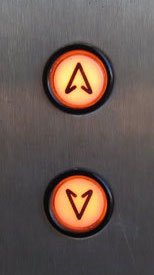
\includegraphics[height=40mm]{img/elevator.jpg}
\end{frame}

\begin{frame}
  \frametitle{Lifts}
  \begin{block}{Algorithm 1}
    Go to the nearest floor that is selected.
  \end{block}
  \centering
  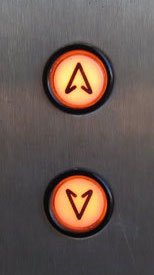
\includegraphics[height=40mm]{img/elevator.jpg}
\end{frame}

\begin{frame}
  \vspace{-16mm}
  \begin{block}{Algorithm 1}
    Go to the nearest floor that is selected.
  \end{block}
  \vspace{5mm}
  \begin{variableblock}{Bug report}{bg=stone,fg=black}{bg=black,fg=white}
    \begin{itemize}
    \item Under certain workloads, people in the lift starve to death before they reach the destination floor.
    \end{itemize}
  \end{variableblock}
\end{frame}

\begin{frame}
  \vspace{-16mm}
  \begin{block}{Algorithm 1}
    Go to the nearest floor that is selected.
  \end{block}
  \centering
  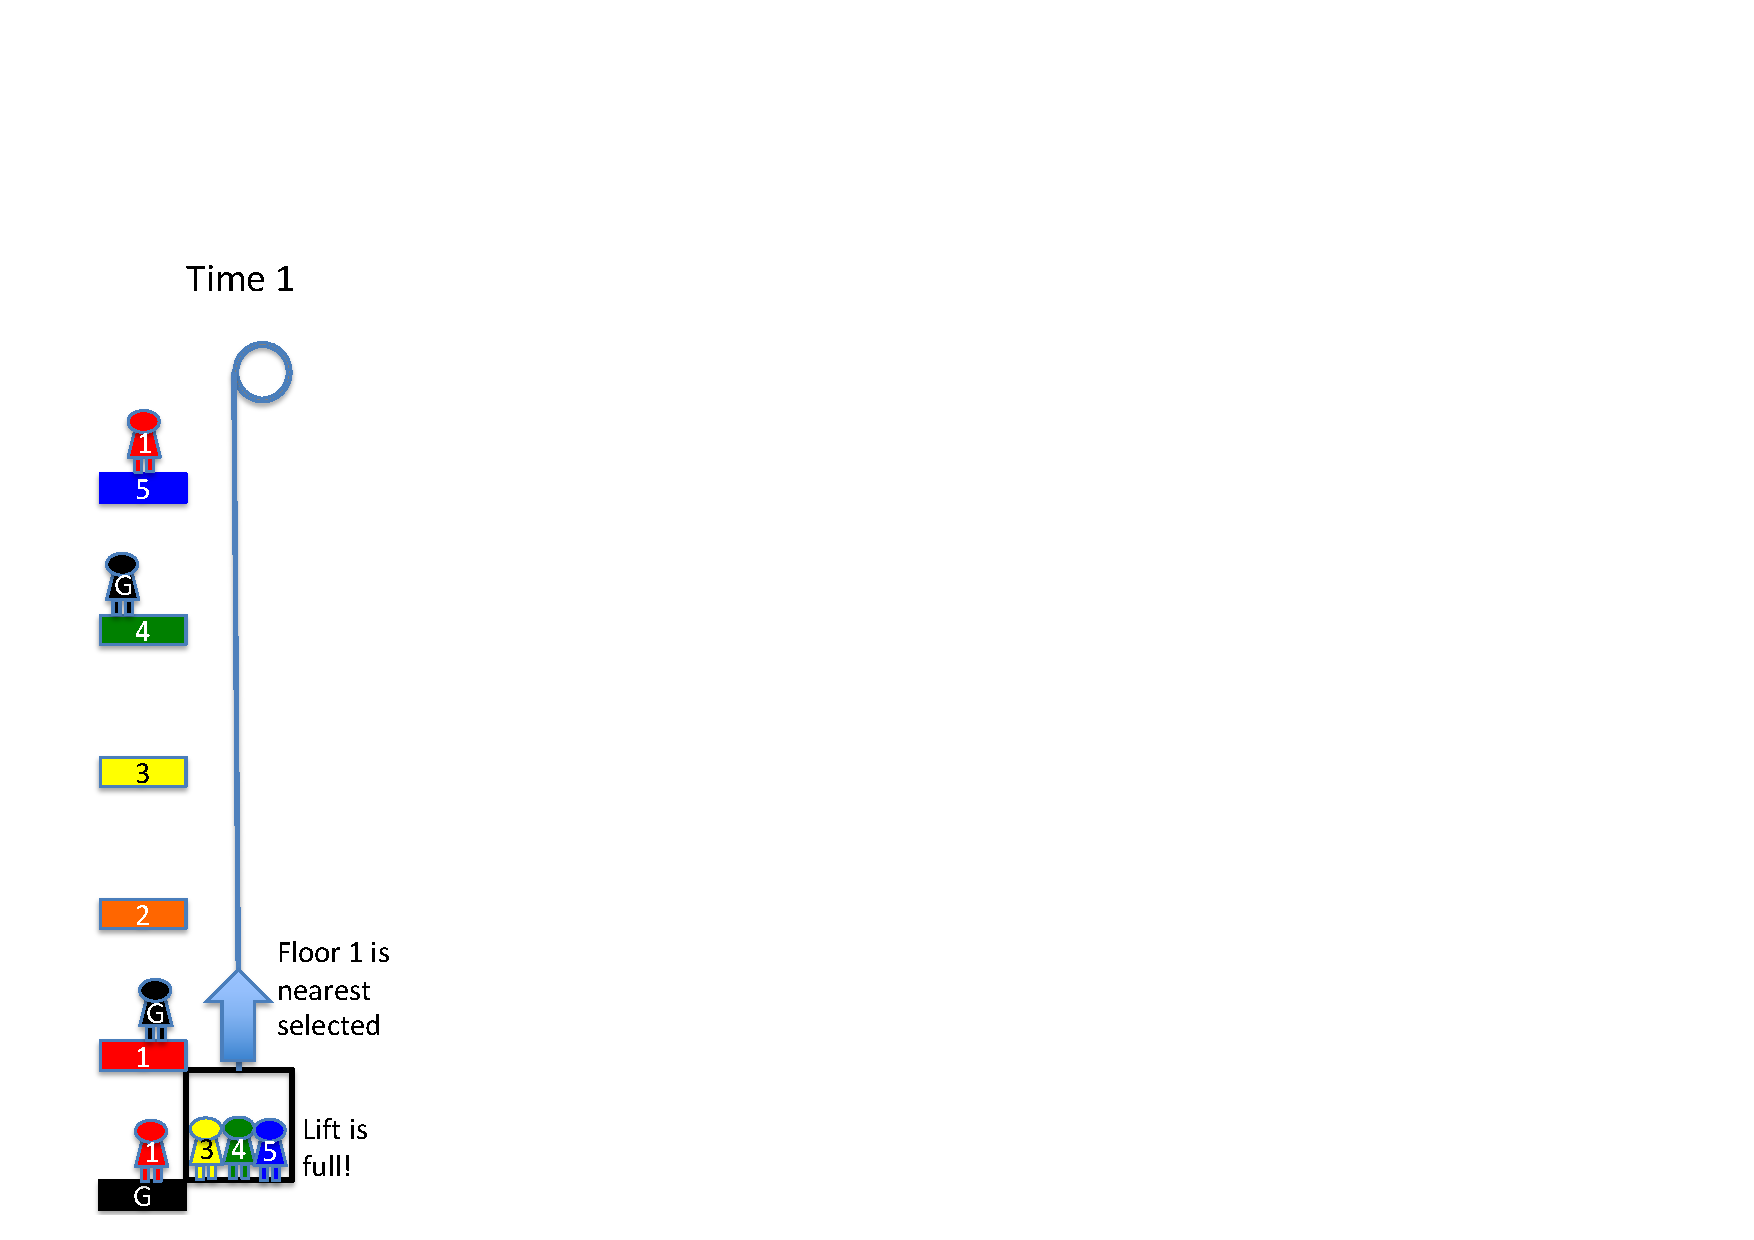
\includegraphics[width=120mm, trim=0mm 0mm 0mm 50mm, clip=true]{img/lift2-anim1.pdf}

\end{frame}

\begin{frame}
  \vspace{-16mm}
  \begin{block}{Algorithm 1}
    Go to the nearest floor that is selected.
  \end{block}
  \centering
  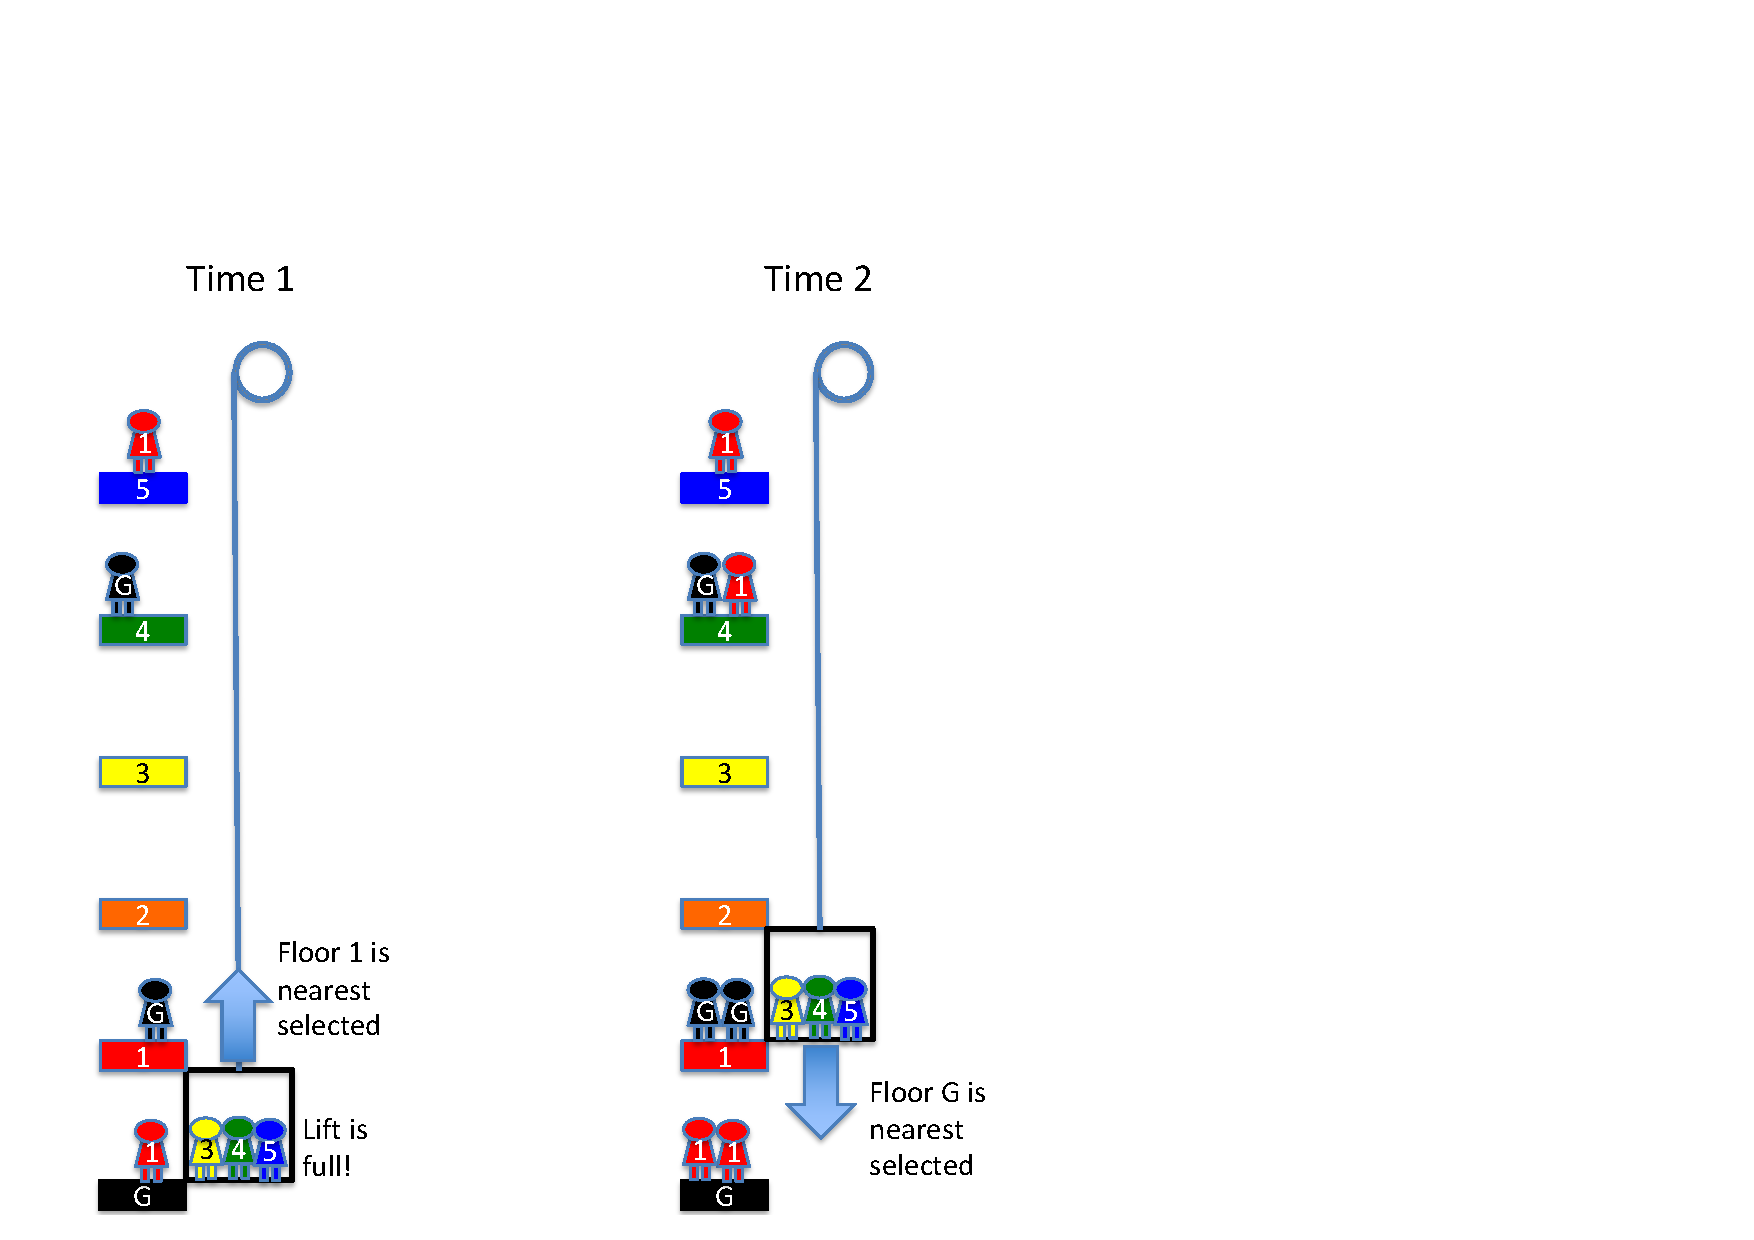
\includegraphics[width=120mm, trim=0mm 0mm 0mm 50mm, clip=true]{img/lift2-anim2.pdf}

\end{frame}

\begin{frame}
  \vspace{-16mm}
  \begin{block}{Algorithm 1}
    Go to the nearest floor that is selected.
  \end{block}
  \centering
  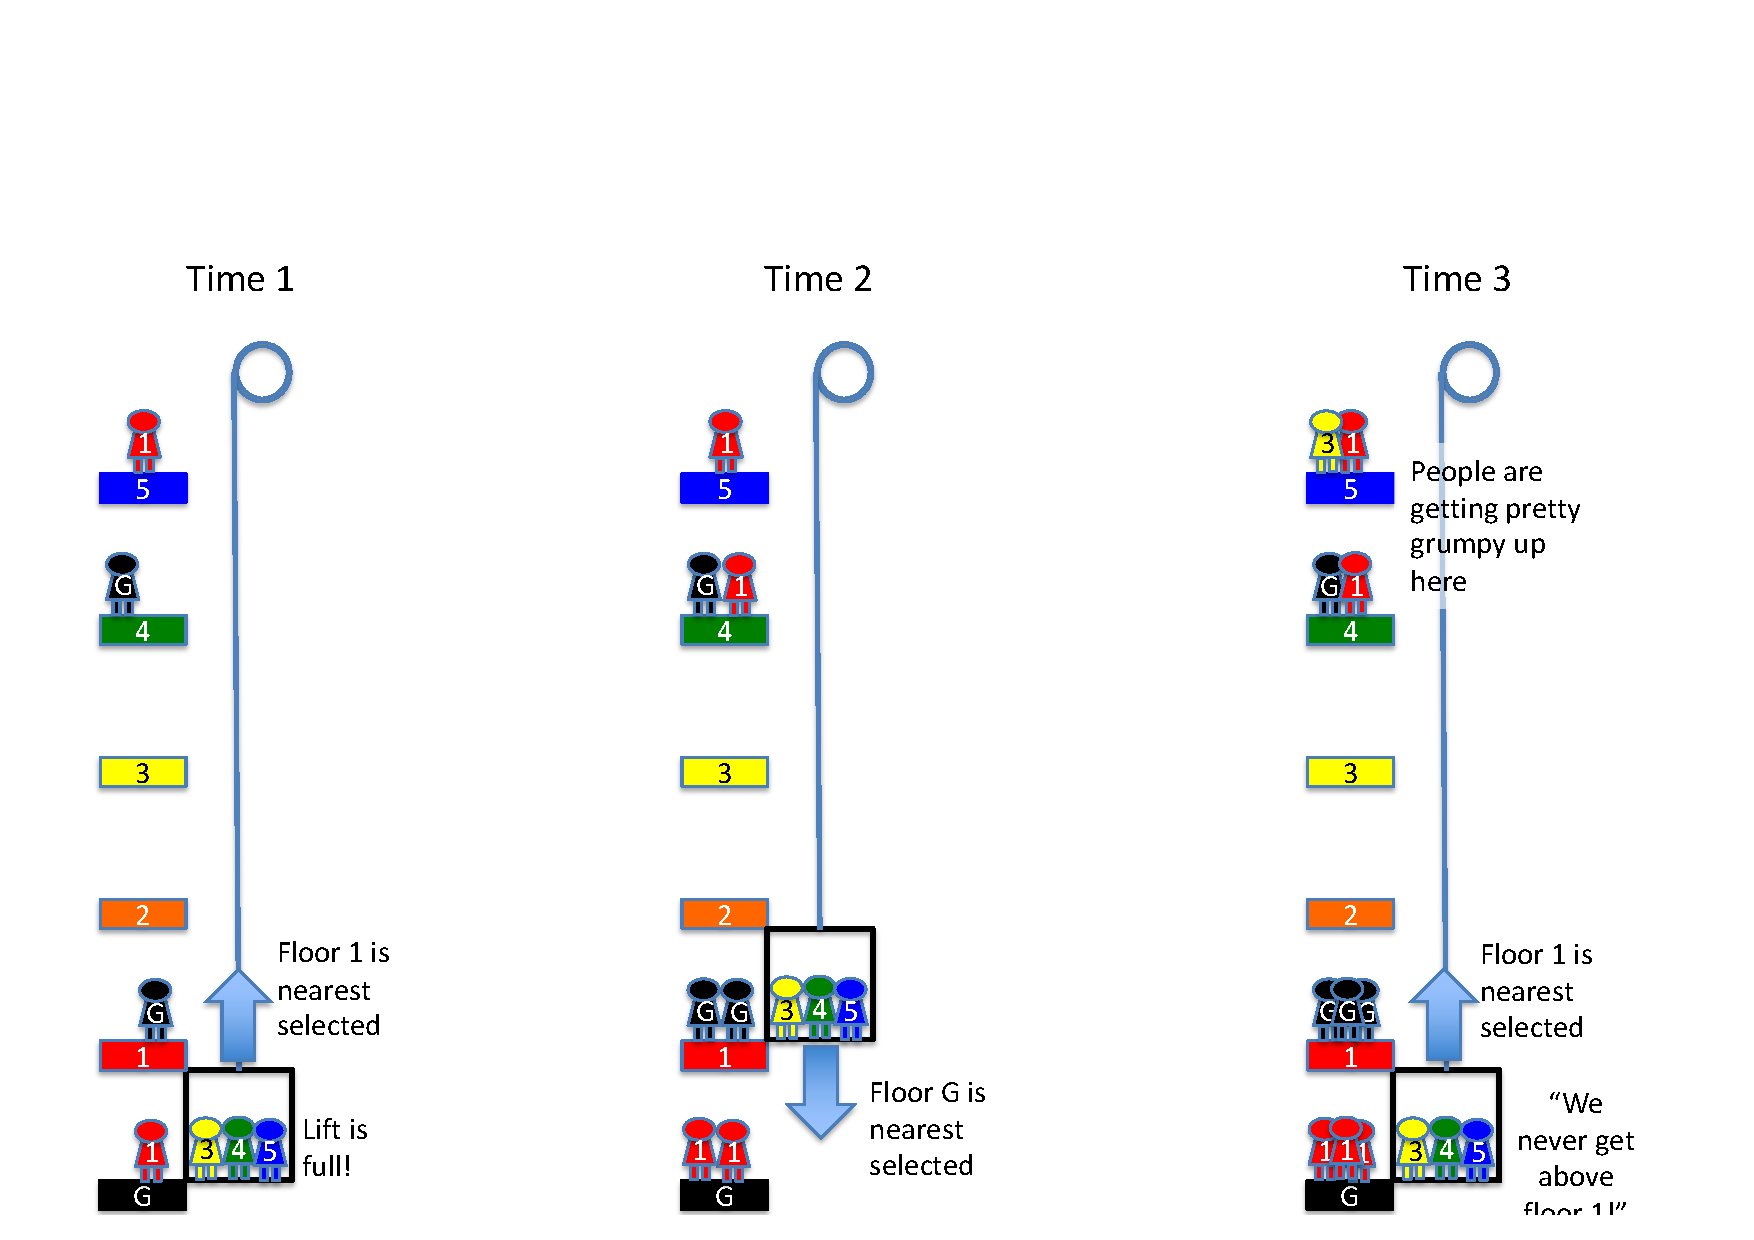
\includegraphics[width=120mm, trim=0mm 0mm 0mm 50mm, clip=true]{img/lift2-anim3.pdf}

\end{frame}

\begin{frame}
  %\vspace{-16mm}
  \begin{block}{Algorithm 1}
    Go to the nearest floor that is selected.
  \end{block}
  \vspace{5mm}
  \begin{variableblock}{Bug report}{bg=stone,fg=black}{bg=black,fg=white}
    \begin{itemize}
    \item Under certain workloads, people in the lift starve to death before they reach the destination floor.
    \end{itemize}
  \end{variableblock}
  \vspace{5mm}
  \begin{block}{Diagnosis}
    Need to prioritse going to the floor selected by people in the lift.
  \end{block}
\end{frame}

\begin{frame}
  \frametitle{Lifts}
  \begin{block}{Algorithm 2}
    \begin{itemize}
    \item Go to the nearest floor selected by people in the lift.
    \item If no floor selected in the lift, go to nearest floor where someone has pressed a call button.
    \end{itemize}
  \end{block}
  \centering
  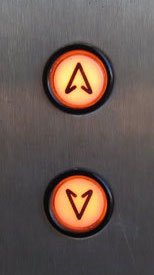
\includegraphics[height=40mm]{img/elevator.jpg}
\end{frame}

\begin{frame}
  \begin{block}{Algorithm 2}
    \begin{itemize}
    \item Go to the nearest floor selected by people in the lift.
    \item If no floor selected in the lift, go to nearest floor where someone has pressed a call button.
    \end{itemize}
  \end{block}
  \vspace{5mm}
  \begin{variableblock}{Bug report}{bg=stone,fg=black}{bg=black,fg=white}
    \begin{itemize}
    \item Under certain workloads, people waiting for the lift starve to death because the lift always goes past their floor.
    \end{itemize}
  \end{variableblock}
\end{frame}


\begin{frame}
  \vspace{-10mm}
  \begin{block}{Algorithm 2}
    \begin{itemize}
    \item Go to the nearest floor selected by people in the lift.
    \item If no floor selected in the lift, go to nearest floor where someone has pressed a call button.
    \end{itemize}
  \end{block}
  \centering
  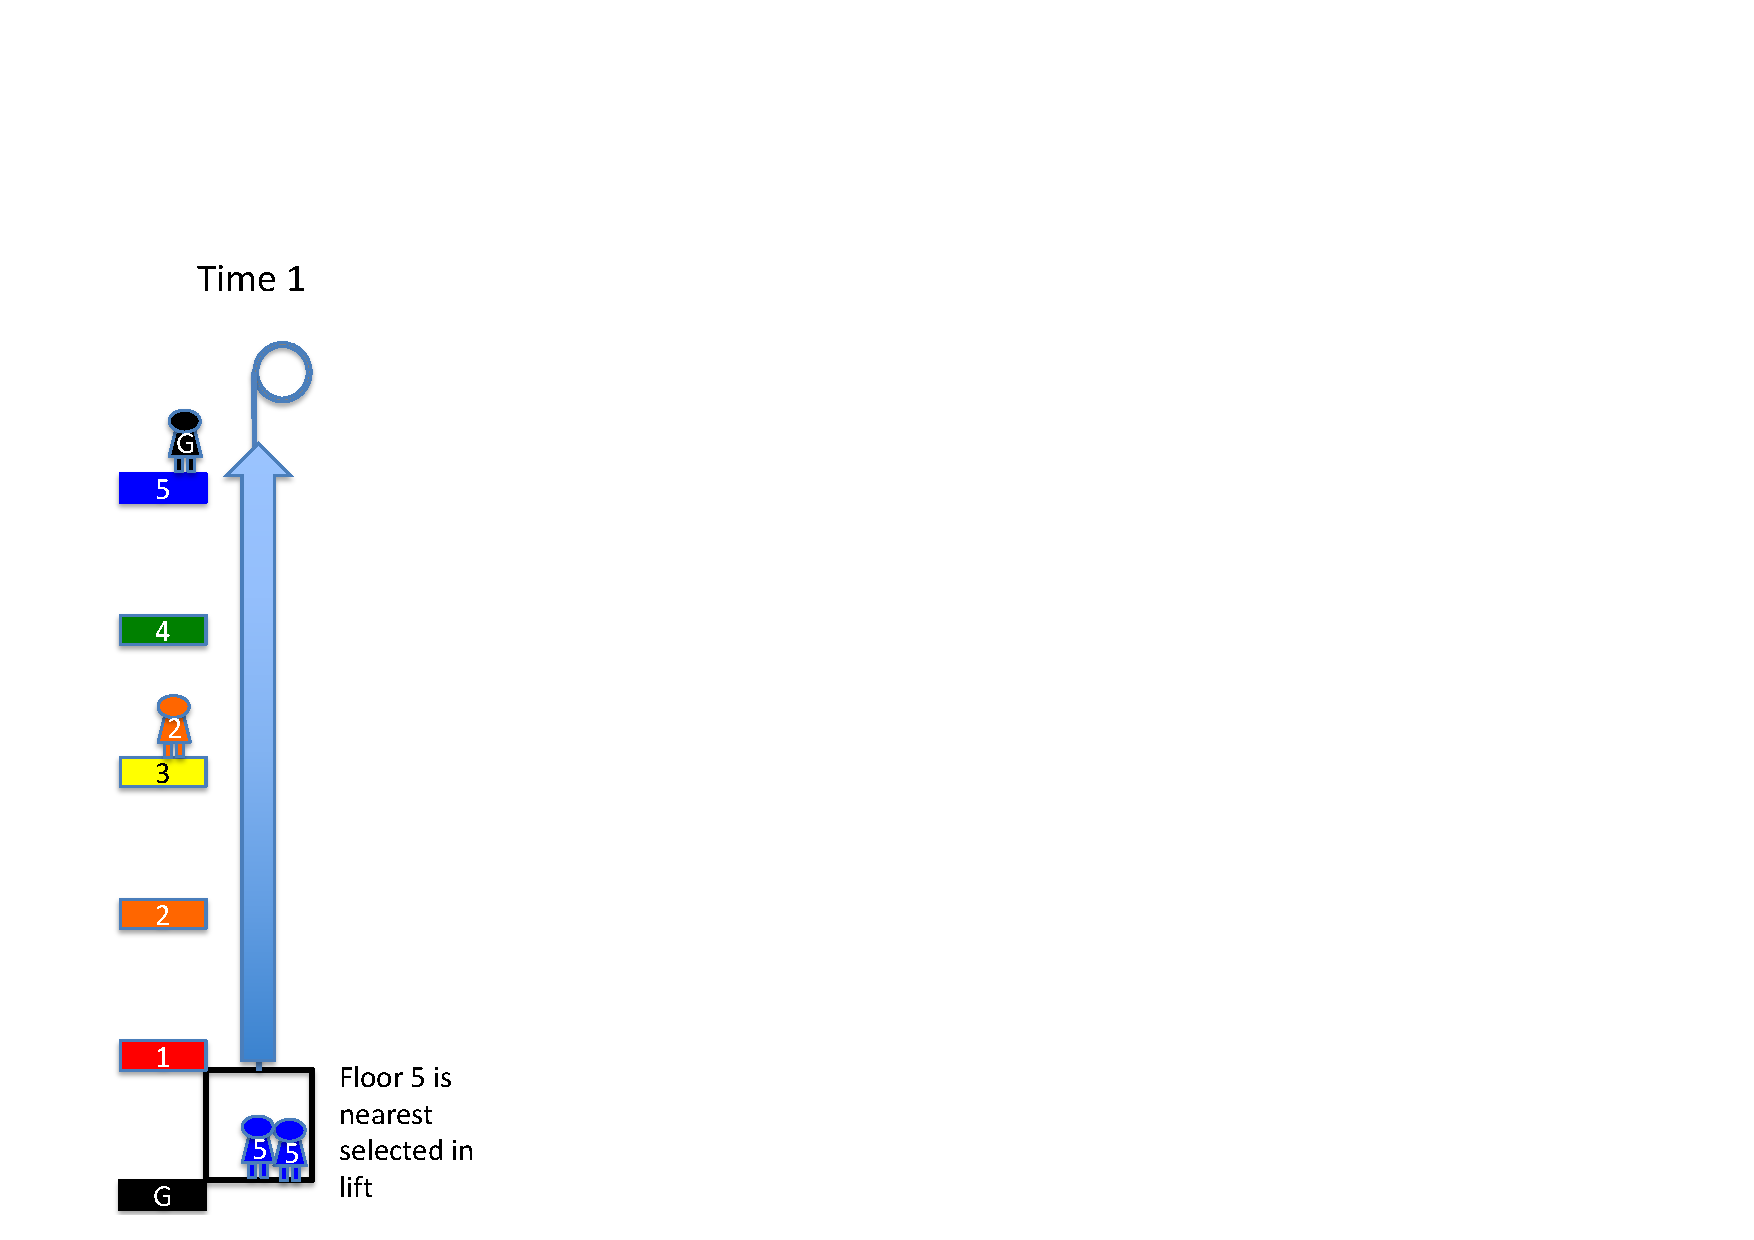
\includegraphics[width=120mm, trim=0mm 0mm 0mm 50mm, clip=true]{img/lift2-anim4.pdf}

\end{frame}

\begin{frame}
  \vspace{-10mm}
  \begin{block}{Algorithm 2}
    \begin{itemize}
    \item Go to the nearest floor selected by people in the lift.
    \item If no floor selected in the lift, go to nearest floor where someone has pressed a call button.
    \end{itemize}
  \end{block}
  \centering
  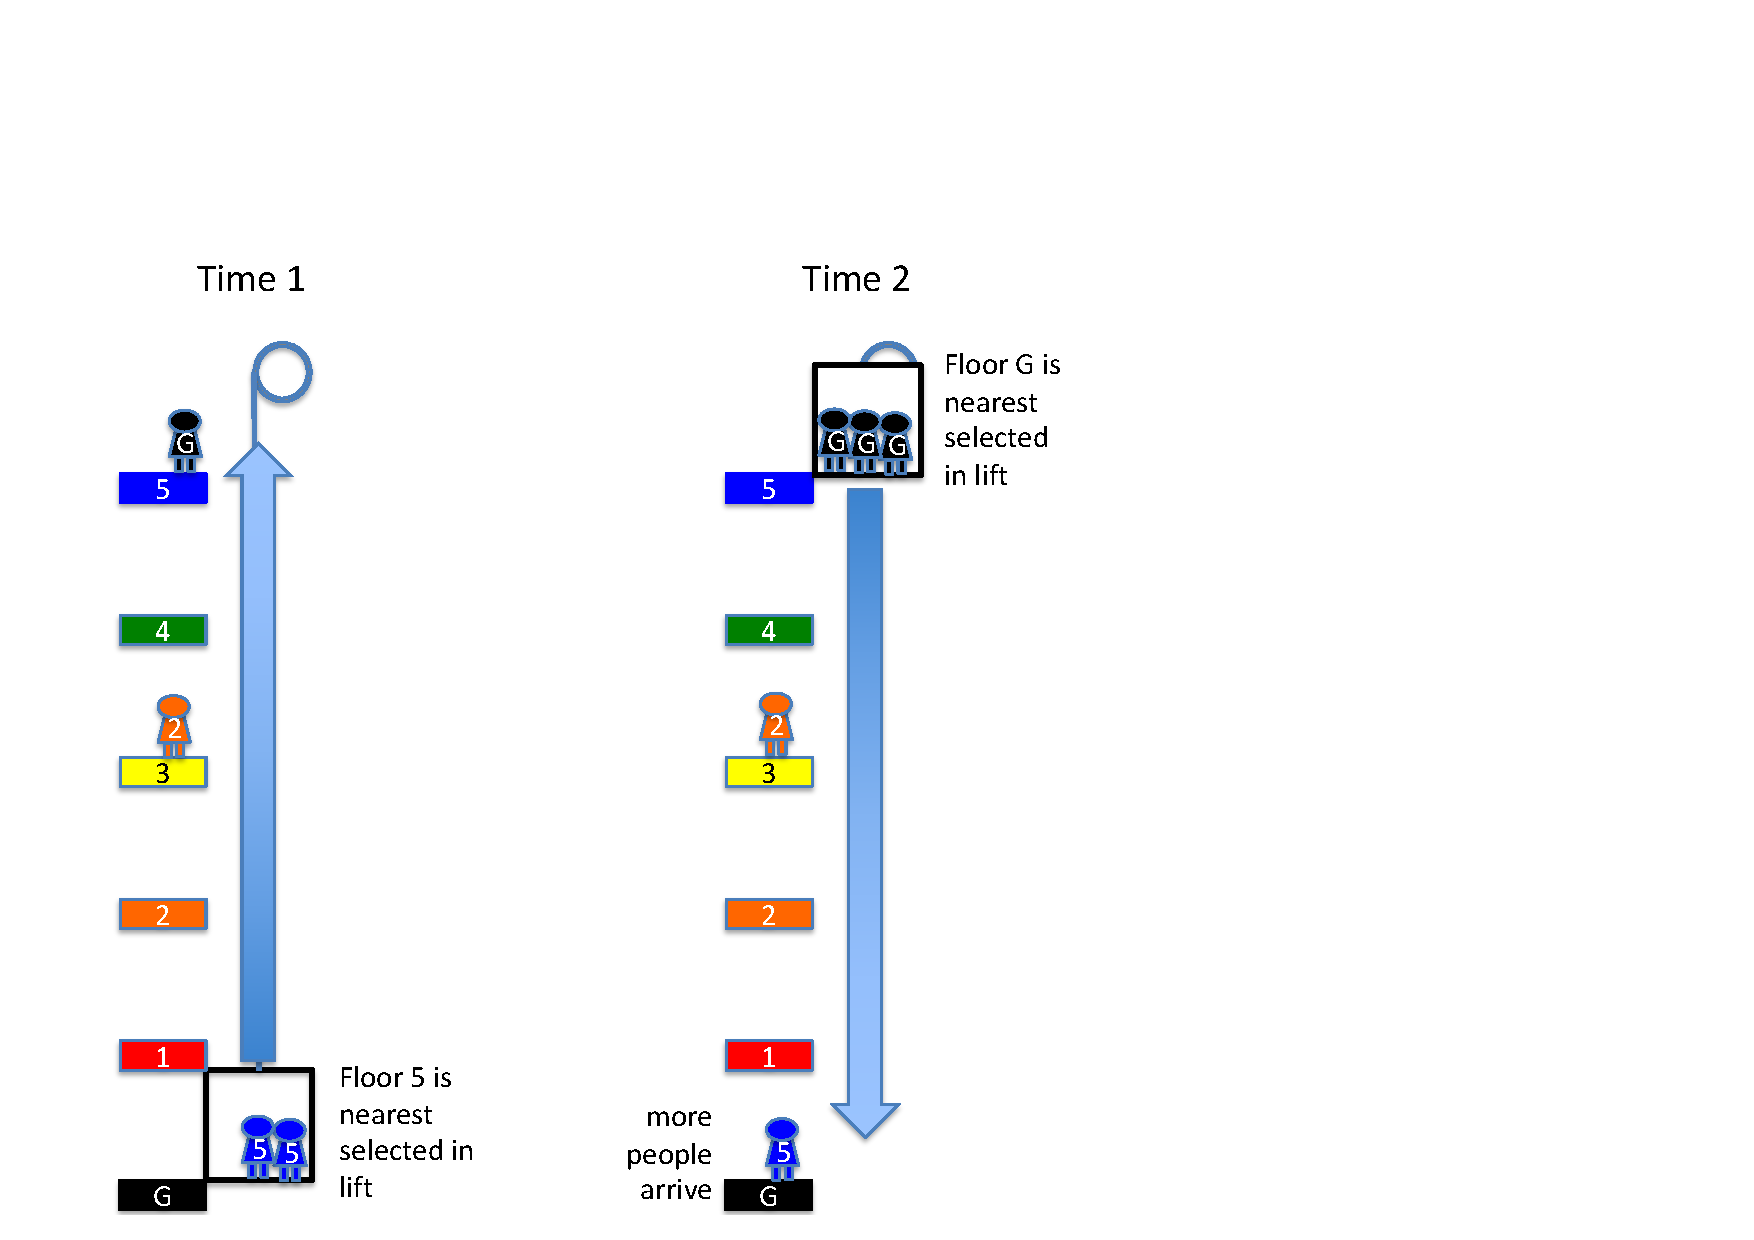
\includegraphics[width=120mm, trim=0mm 0mm 0mm 50mm, clip=true]{img/lift2-anim5.pdf}
\end{frame}

\begin{frame}
  \vspace{-10mm}
  \begin{block}{Algorithm 2}
    \begin{itemize}
    \item Go to the nearest floor selected by people in the lift.
    \item If no floor selected in the lift, go to nearest floor where someone has pressed a call button.
    \end{itemize}
  \end{block}
  \centering
  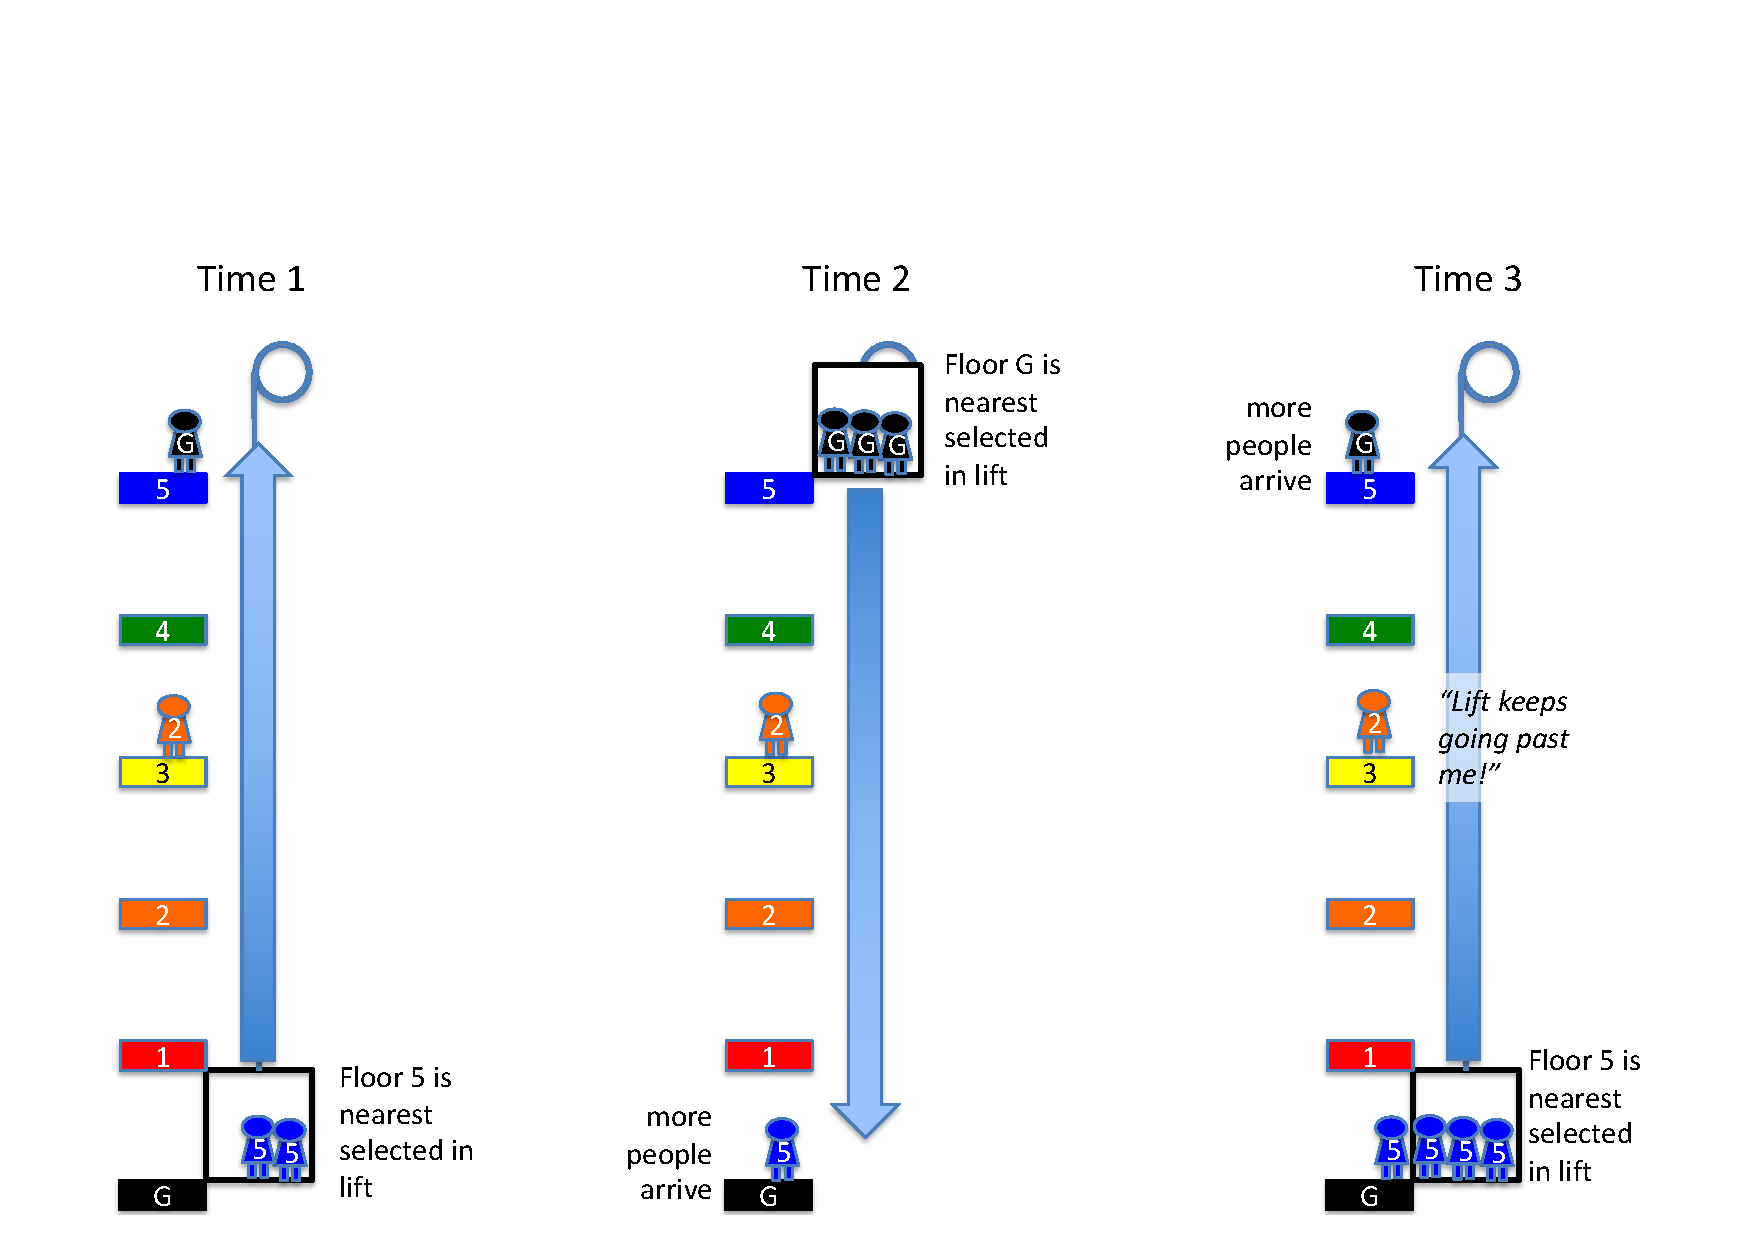
\includegraphics[width=120mm, trim=0mm 0mm 0mm 50mm, clip=true]{img/lift2-anim6.pdf}
\end{frame}

\begin{frame}
  \vspace{-2mm}
  \begin{block}{Algorithm 2}
    \begin{itemize}
    \item Go to the nearest floor selected by people in the lift.
    \item If no floor selected in the lift, go to nearest floor where someone has pressed a call button.
    \end{itemize}
  \end{block}
  \vspace{1mm}
  \begin{variableblock}{Bug report}{bg=stone,fg=black}{bg=black,fg=white}
    \begin{itemize}
    \item Under certain workloads, people in the lift starve to death before they reach the destination floor.
    \end{itemize}
  \end{variableblock}
  \vspace{1mm}
  \begin{block}{Diagnosis}
    Should not skip a floor where someone wants to go in the direction the lift is going.
  \end{block}
\end{frame}

\begin{frame}
  \begin{block}{Algorithm 3}
    \begin{itemize}
      \item Go to the next floor selected by people in the lift, but don't go past a floor where someone wants to go in the same direction the lift is going.
      \item If no floor is selected, go to the nearest floor where someone has pressed a button.
    \end{itemize}
  \end{block}
  \centering
  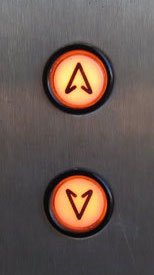
\includegraphics[height=40mm]{img/elevator.jpg}
\end{frame}

\begin{frame}
  \begin{block}{Algorithm 3}
    \begin{itemize}
      \item Go to the next floor selected by people in the lift, but don't go past a floor where someone wants to go in the same direction the lift is going.
      \item If no floor is selected, go to the nearest floor where someone has pressed a button.
    \end{itemize}
  \end{block}
  \vspace{5mm}
  \begin{variableblock}{Bug report}{bg=stone,fg=black}{bg=black,fg=white}
    \begin{itemize}
    \item Under certain workloads, people in the lift starve to death before they reach the destination floor.
    \end{itemize}
  \end{variableblock}
\end{frame}

\begin{frame}
  \vspace{-11mm}
  \begin{block}{Algorithm 3}
    \begin{itemize}
      \vspace{-1mm}
      \item \small Go to the next floor selected by people in the lift, but don't go past a floor where someone wants to go in the same direction the lift is going.
      \vspace{-1mm}
      \item \small If no floor is selected, go to the nearest floor where someone has pressed a button.
      \vspace{-1mm}
    \end{itemize}
  \end{block}
  \centering
  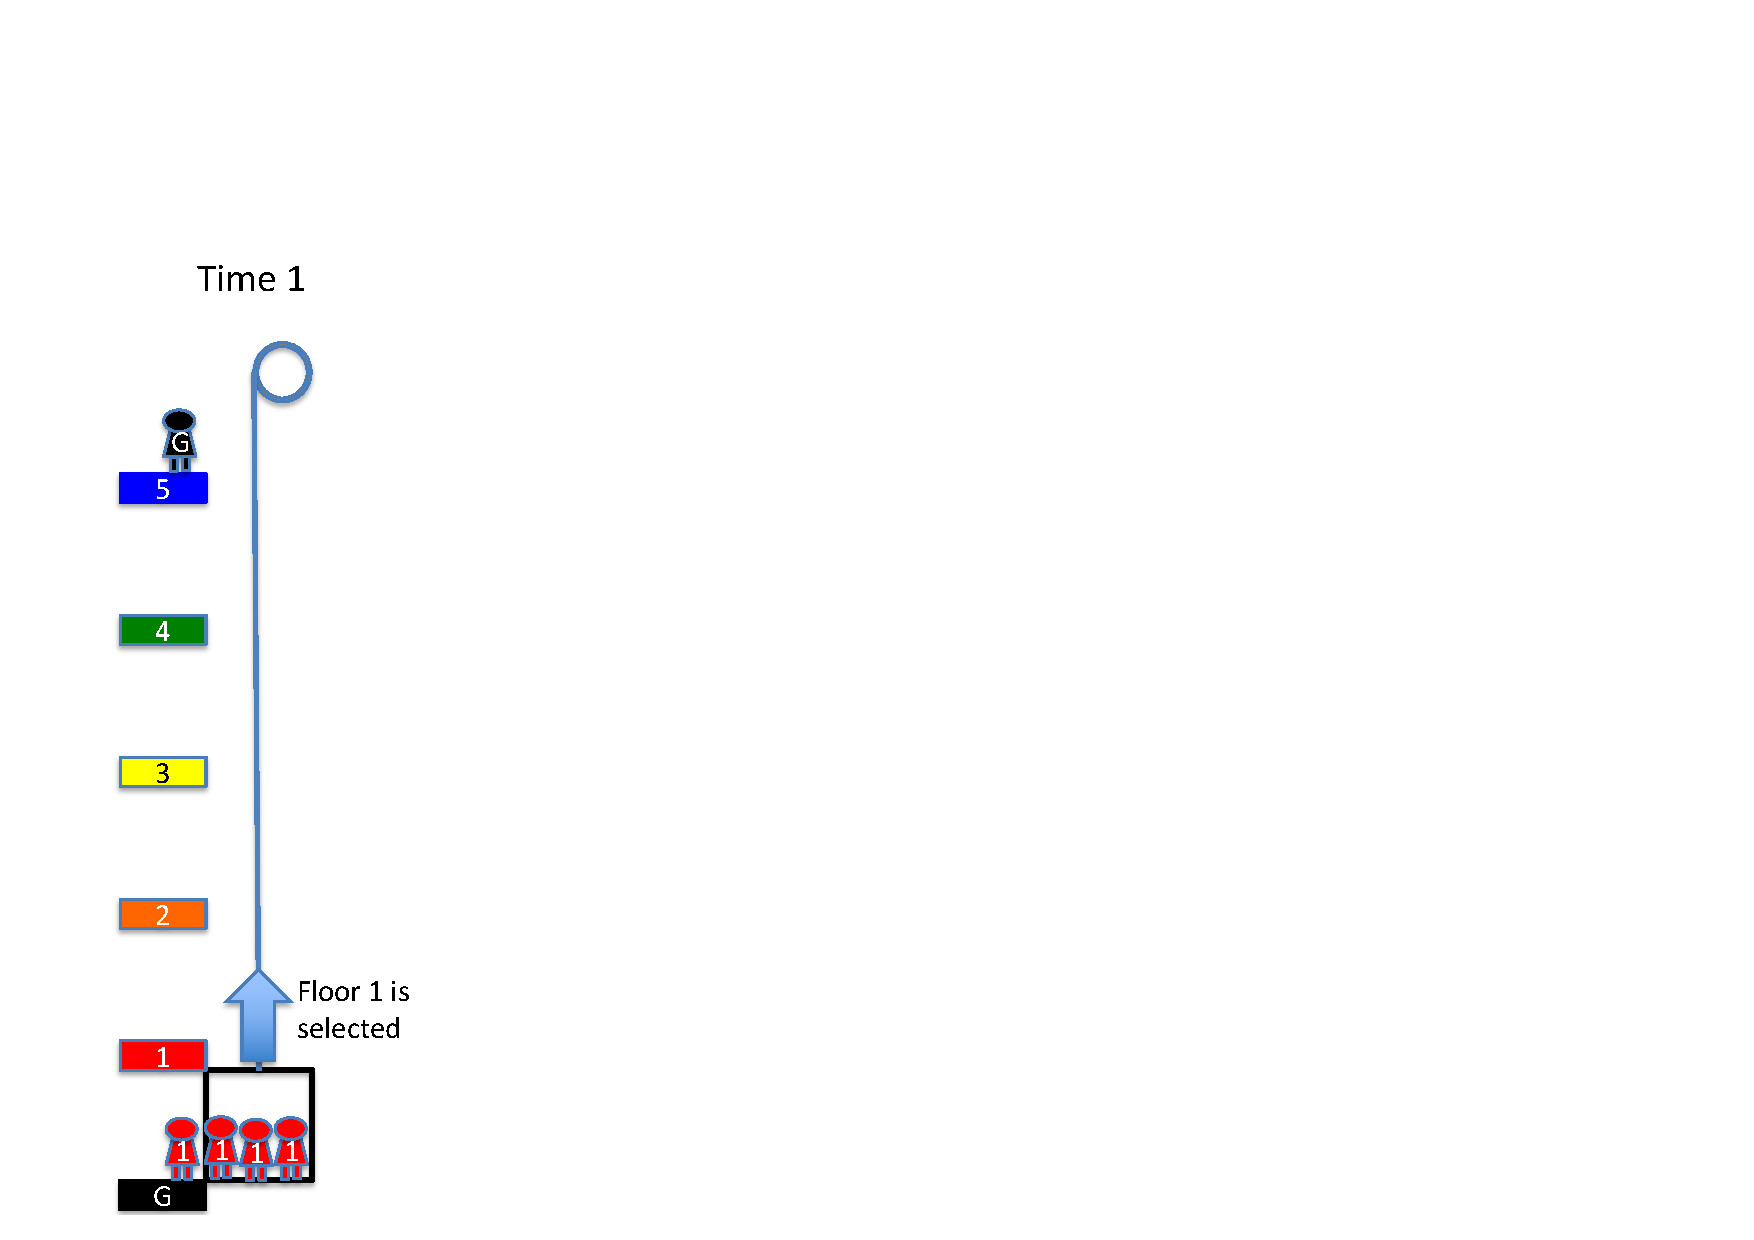
\includegraphics[width=120mm, trim=0mm 0mm 0mm 50mm, clip=true]{img/lift2-anim7.pdf}

\end{frame}

\begin{frame}
  \vspace{-11mm}
  \begin{block}{Algorithm 3}
    \begin{itemize}
      \vspace{-1mm}
      \item \small Go to the next floor selected by people in the lift, but don't go past a floor where someone wants to go in the same direction the lift is going.
      \vspace{-1mm}
      \item \small If no floor is selected, go to the nearest floor where someone has pressed a button.
      \vspace{-1mm}
    \end{itemize}
  \end{block}
  \centering
  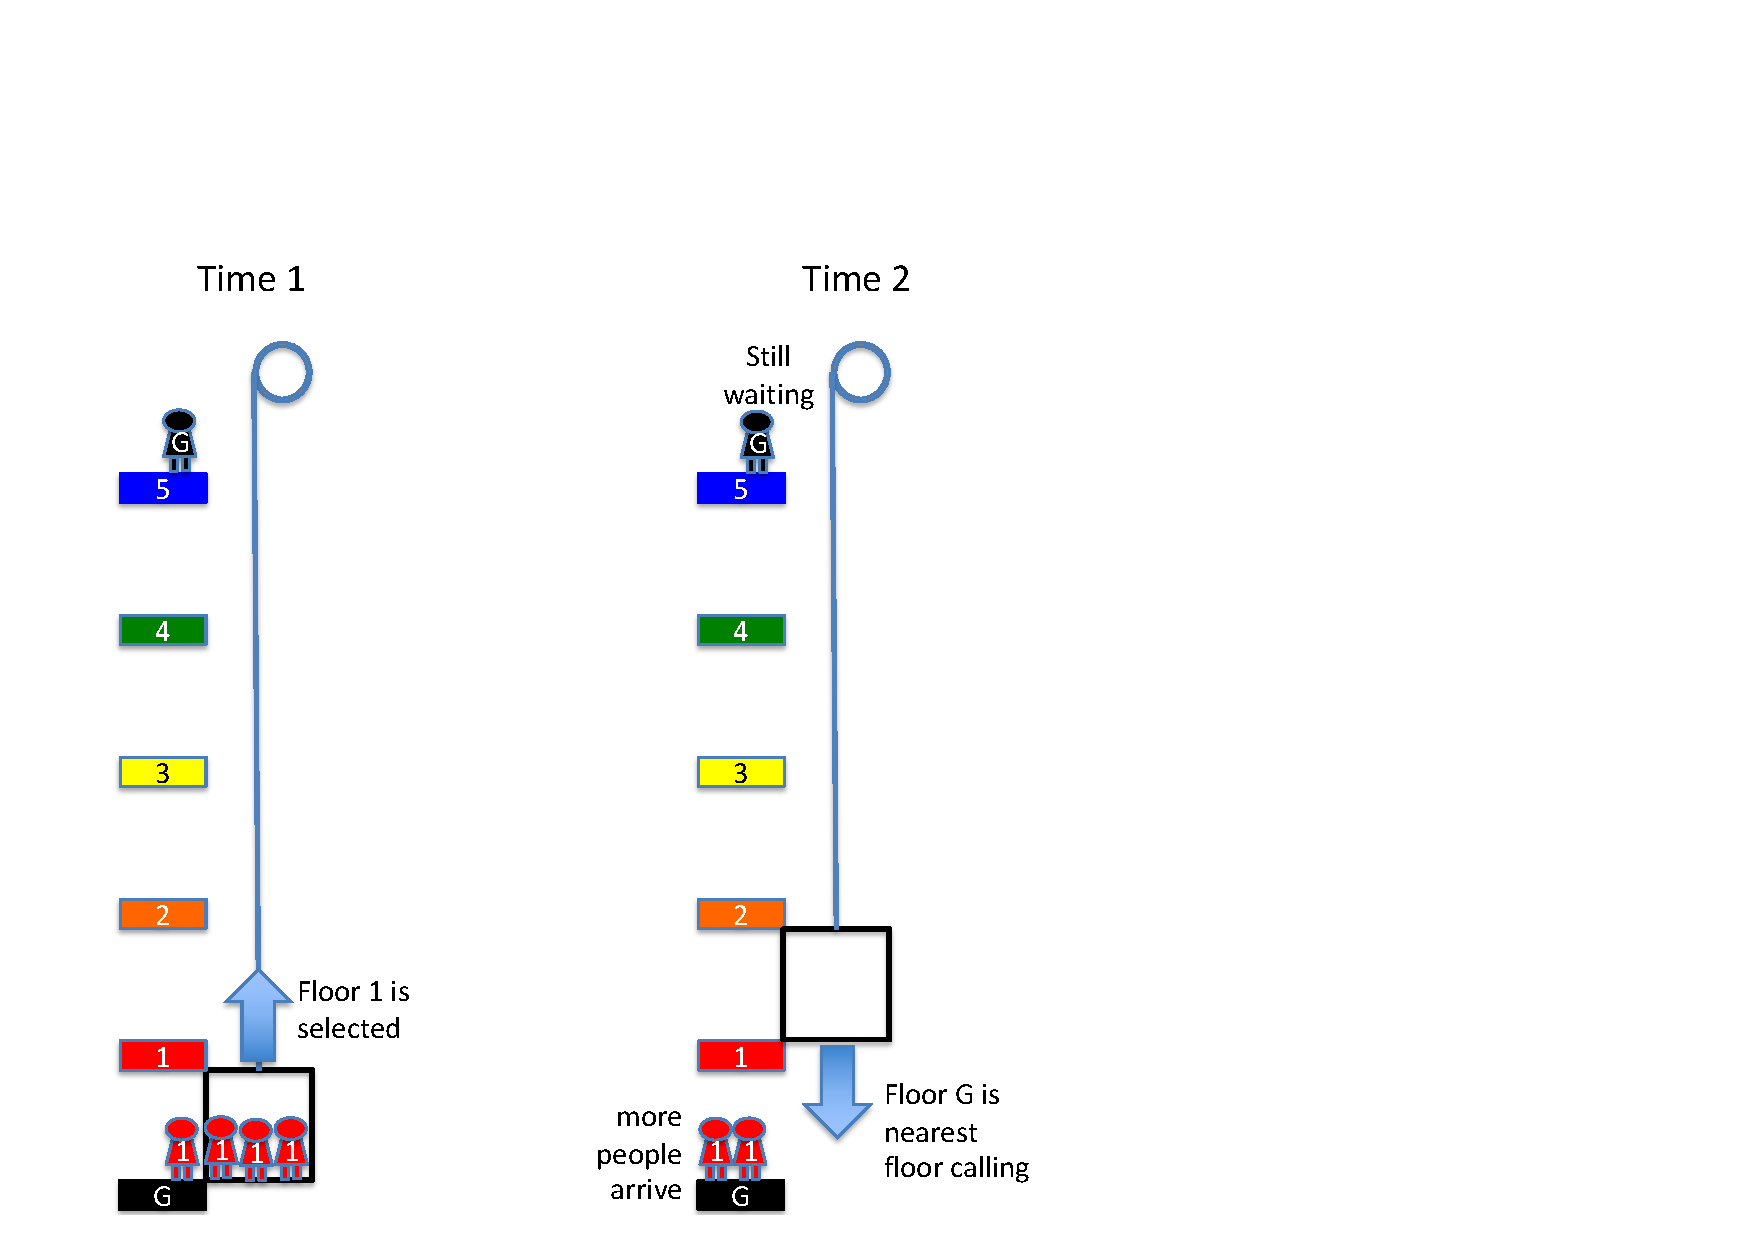
\includegraphics[width=120mm, trim=0mm 0mm 0mm 50mm, clip=true]{img/lift2-anim8.pdf}

\end{frame}

\begin{frame}
  \vspace{-11mm}
  \begin{block}{Algorithm 3}
    \begin{itemize}
      \vspace{-1mm}
      \item \small Go to the next floor selected by people in the lift, but don't go past a floor where someone wants to go in the same direction the lift is going.
      \vspace{-1mm}
      \item \small If no floor is selected, go to the nearest floor where someone has pressed a button.
      \vspace{-1mm}
    \end{itemize}
  \end{block}
  \centering
  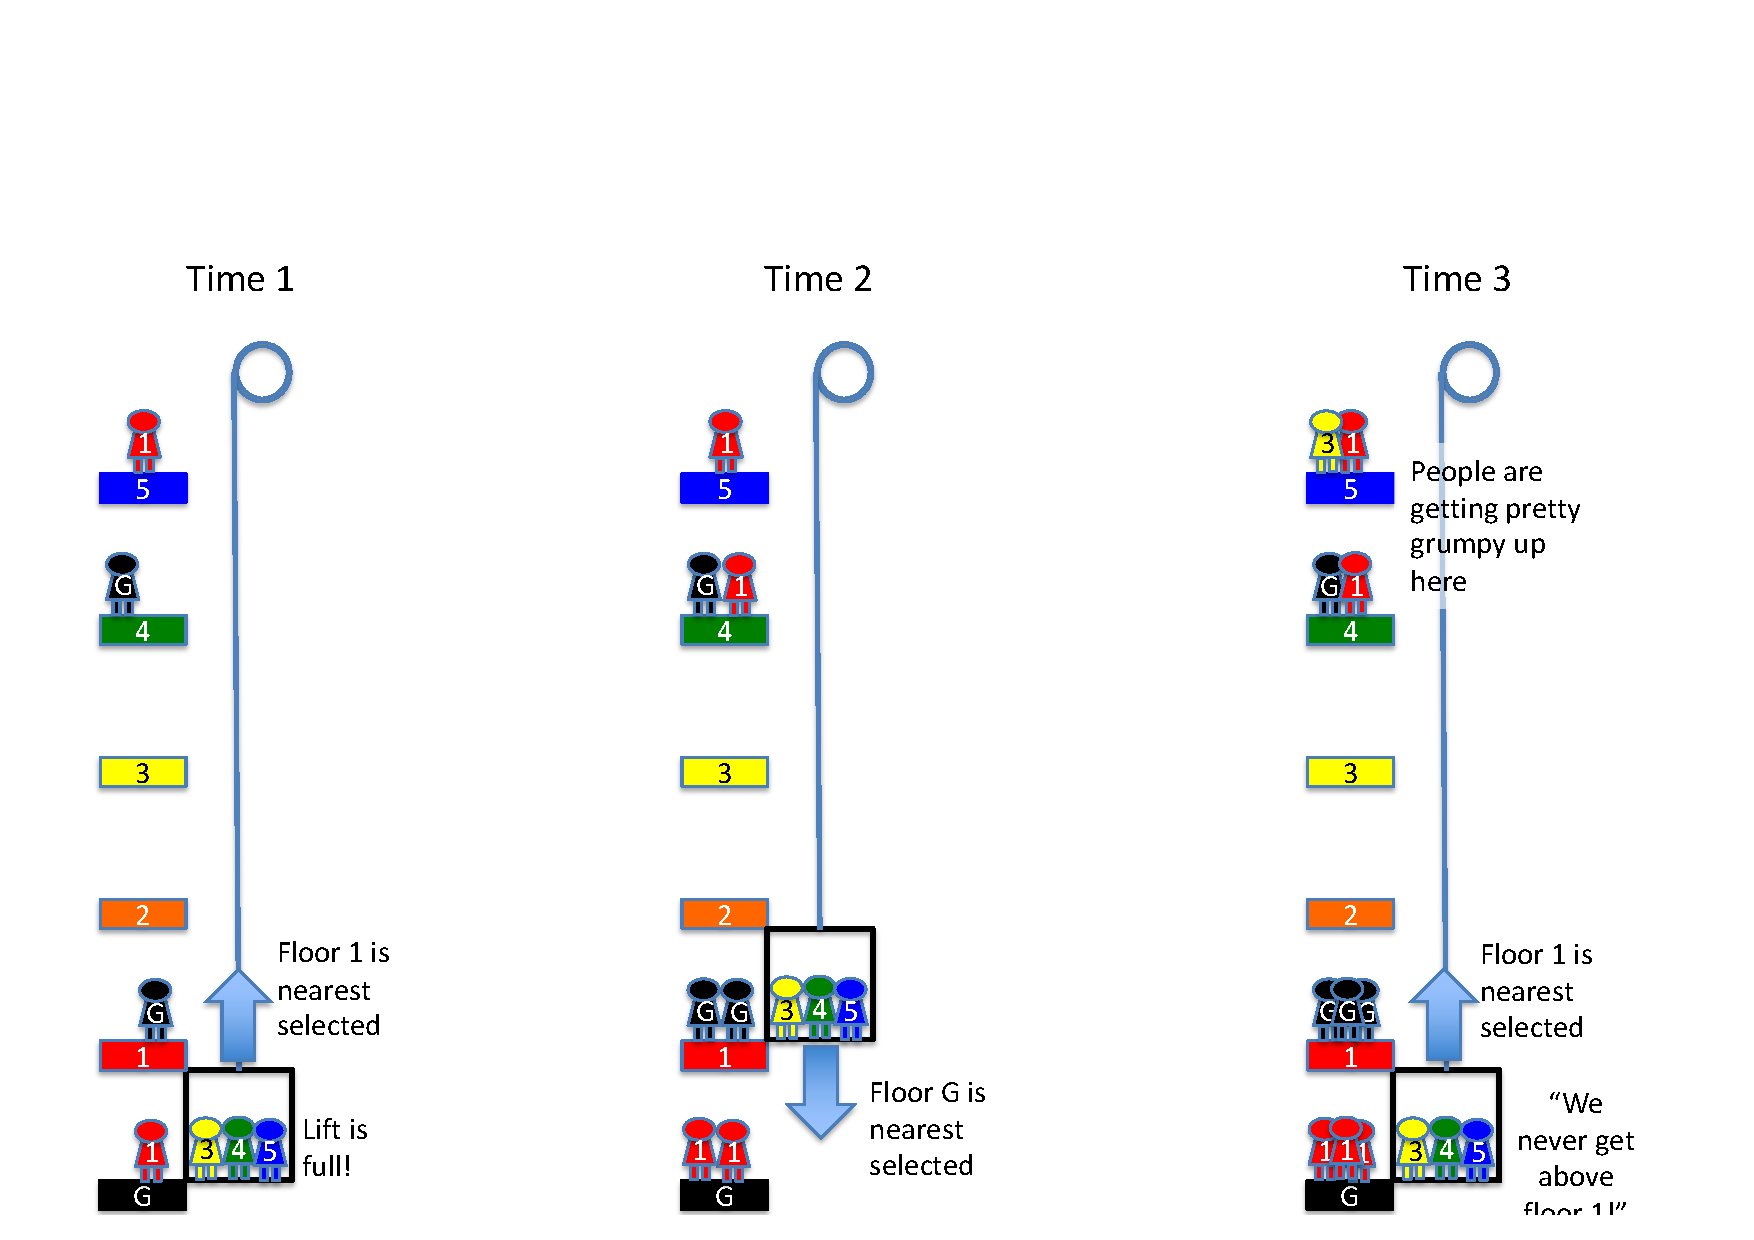
\includegraphics[width=120mm, trim=0mm 0mm 0mm 50mm, clip=true]{img/lift2-anim3.pdf}

\end{frame}

\begin{frame}
  \begin{block}{Algorithm 3}
    \begin{itemize}
      \item Go to the next floor selected by people in the lift, but don't go past a floor where someone wants to go in the same direction the lift is going.
      \item If no floor is selected, go to the nearest floor where someone has pressed a button.
    \end{itemize}
  \end{block}
  \vspace{5mm}
  \begin{variableblock}{Bug report}{bg=stone,fg=black}{bg=black,fg=white}
    \begin{itemize}
    \item Under certain workloads, people in the lift starve to death before they reach the destination floor.
    \end{itemize}
  \end{variableblock}
  \vspace{1mm}
  \begin{block}{Diagnosis}
    Lift should not turn round if it's heading towards people who are waiting.
  \end{block}
\end{frame}

\begin{frame}
  \begin{block}{Algorithm 4}
    \begin{itemize}
    \item Go in one direction, stopping at floors where:
      \begin{itemize}
      \item people outside want to go in that direction, or
      \item where people in the lift want to go in that direction.
        \end{itemize}
       \item Change direction only when there are no more selected floors or call buttons pressed in that direction.
    \end{itemize}
  \end{block}
  \centering
  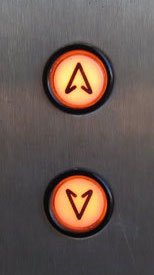
\includegraphics[height=40mm]{img/elevator.jpg}
\end{frame}

  
\begin{frame}
  \begin{block}{Algorithm 4}
    \begin{itemize}
    \item Go in one direction, stopping at floors where:
      \begin{itemize}
      \item people outside want to go in that direction, or
      \item where people in the lift want to go in that direction.
        \end{itemize}
       \item Change direction only when there are no more selected floors or call buttons pressed in that direction.
    \end{itemize}
  \end{block}
  \vspace{5mm}
  \begin{variableblock}{Bug reports}{bg=stone,fg=black}{bg=black,fg=white}
    \begin{itemize}
    \item --- NO BUG REPORTS FILED ---
    \end{itemize}
  \end{variableblock}
\end{frame}

  
\begin{frame}
  \begin{block}{Challenge 1}
    \begin{itemize}
    \item What should the lift do if no call button is pressed?
    \end{itemize}
  \end{block}
  \centering
  \begin{block}{Challenge 2}
    \begin{itemize}
    \item Extend the algorithm so it works efficiently to control two lifts.
    \end{itemize}
  \end{block}
  \centering
  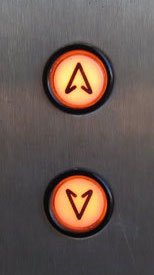
\includegraphics[height=40mm]{img/elevator.jpg}
\end{frame}



\begin{frame}
\frametitle{Euclid's algorithm for computing the GCD. (I)} 

Euclid of Alexandria (300 BC) was interested in properties of integer and rational numbers. 

\vspace{5mm}
Finding the \emc{greatest common denominator} (GCD) allowed them to simplify fractions:

\vspace{5mm}
Eg.\ $\frac{390253}{228769} = \frac{29 \cdot 13457}{17 \cdot 13457} = \frac{29}{17}$ since $GCD(390253, 228769) = 13457$.

\vspace{5mm}
But how to compute the GCD function without resorting to factoring the numbers (which turns out to be a hard problem for large numbers)?

\end{frame}

\begin{frame}
\frametitle{Euclid's algorithm for computing the GCD. (II)} 

\begin{block}{Euclid's algorithm for computing the GCD (in prose)}
\begin{itemize}
\item Consider the two integers for which you want to find the GCD.
\item Take the smaller one, and subtract it from the larger one. 
\item Replace the larger one with this result, and keep the smaller one, as your two new numbers. 
\item Repeat until the two numbers are equal. 
\item Once they are, the resulting (equal) numbers are the GCD.  
\end{itemize}
\end{block}

Let's build a Python program where we execute the concrete steps of the algorithm for the sample numbers 42 and 30.

\end{frame}

\begin{frame}
\frametitle{Why Euclid's algorithm works? (I)}

Consider the positive integers $a$ and $b$; express using $a'$ and $b'$:
\begin{align}
a &= \alpha \cdot gcd(a,b), \\
b &= \beta \cdot gcd(a,b),
\end{align}
where $gcd(\alpha, \beta) = 1.$

Without loss of generality, consider $a > b$. After a single step:
\begin{align}
a' &= a - b \\ 
    &= (\alpha - \beta) \cdot gcd(a,b).
\end{align}

Note that $a'$ is always strictly positive.

\end{frame}

\begin{frame}
\frametitle{Why Euclid's algorithm works? (II)}

We can show that $gcd(a', b) = gcd(a,b)$.

Proof by contradiction: 

\begin{itemize}
\item We know that gcd(a,b) is a factor of both a and b. 
\item So if $gcd(a', b) > gcd(a,b)$ it must be that:
$gcd(\alpha - \beta, \beta) = c > 1$. 
\item Thus we can rewrite $\beta = r \cdot c$ and $\alpha - \beta = r' \cdot c \Leftrightarrow \alpha = (r' + r) \cdot c $. 
\item However that means that $\alpha$ and $\beta$ are both divisible by $c > 1$. \\ Which contradicts $gcd(\alpha, \beta) = 1$.
\end{itemize}

Thus by repeatedly applying the steps of the algorithm we keep the gcd in each step constant while reducing the size of $a$ and $b$. Until they are equal to the gcd.

\end{frame}



\begin{frame}

\frametitle{Calculations following Euclid's algorithm for GCD.} 


	\inputminted[
		xleftmargin=1.4em,
		frame=lines,
		framesep=2mm,
		%baselinestretch=1.2,
		% bgcolor=stone,
		fontsize=\footnotesize,
		linenos
	]{python}{src/interactive_euclid.py}

\end{frame}

\begin{frame}
\frametitle{Assignments, values \& expressions.}

Let's understand all aspects of the Python code in this example.
\begin{itemize}
\item \emc{Statements} perform an action within the program. In this example all code lines are statements.
\item \emc{Assignments} are statements that assign an expression (right hand side of $=$) to a variable with a number in the program (left hand side of $=$). Eg.\ \mint{python}{a = 42} assigns $42$ to the named variable \texttt{a}.
\item \emc{Expressions} are fragments of code that return a computed quantity.
\item \emc{Values} are expressions that return a constant, eg.\ \texttt{42} and \texttt{30.}
\item More generally \emc{arithmetic expressions} such as \texttt{b - a} perform a computation and return its result. They can be nested arbitrarily.
\end{itemize}

\end{frame}

\begin{frame}
\frametitle{Some Python idioms.}

\begin{itemize}
	\item The order of evaluation of arithmetic expressions follows the \emc{usual precedence rules} of integer arithmetic, eg. \texttt{2+3*4} is computed as \texttt{2+(3*4) = 14}. You may force a different order of evaluation by using parenthesis, eg. \texttt{(2+3)*4 = 20}.
	\item Python allows for multiple \emc{simultaneous assignments}. Eg.\ lines 2--3 could be expressed as:
	\mint{python}{a, b = 42, 30}
	All expressions on the right hand-side are first evaluated before any assignment occurs.
	\item Python allows for \emc{reusing names} in the left-hand side of an assignment as in line 10.
	\mint{python}{b = b - a}
	Only \emc{reuse variable names if they represent the same} high-level concept.

\end{itemize}

\end{frame}

\begin{frame}
\frametitle{Types \& Programming Languages. (I)}

Python is a strongly typed and dynamically typed language. 
\begin{itemize}
\item \emc{Strongly typed}: Every variable, or expression has a \emc{type} associated with it. All expressions in our example program are of type \emc{int} representing integers. Only operations supported by this type can be performed on variables or expressions of that type.
\item \emc{Dynamically typed}: While the program runs the types of objects are tracked, and operations are checked before being applied to ensure they are permitted. 
\end{itemize}

\vspace{5mm}
In contract \emc{statically typed} languages run this check before the program executes. However, to decide \emc{type-safety} before execution they \emc{lose expressiveness} or require \emc{type annotations}.

\end{frame}

\begin{frame}
\frametitle{Types \& Programming Languages. (II)}

\begin{block}{Types and formal methods}
Type systems are the most popular \emc{formal methods} that aid program correctness. They ensure only permissible operations are executed, and eliminate a large number of potential trivial bugs. But are \emc{not a substitute for testing} or further \emc{verification} for correctness.
\end{block}

\end{frame}

\begin{frame}
\frametitle{The Python \texttt{int} integer type} 

The type \emc{int} is primitive, in that the Python language itself knows about it out of the box. It can represent \emc{integers of arbitrary length} (unlike other languages), and supports:
\begin{itemize}
\item The arithmetic operators $+$, $-$, $*$ and $**$ (to the power) return integers.
\item The integer division $//$ and remainder operator $\%$ also return integers.
\item Division, but does not return an integer!
\item The function \texttt{int(x)} returns the integer representation of \texttt{x} (if it exists).
\end{itemize}

\end{frame}

\begin{frame}
\frametitle{Primitive and user-defined types} 

Python supports out-of-the-box a number of types, including integers, complex numbers, real numbers (\texttt{float}), truth values (\texttt{bool}), strings of characters (\texttt{str}), and many data structures.

\vspace{5mm}
A \emc{full list of all supported operations} can be found in the documentation for all primitive types. \emc{Study it} carefully. \url{https://docs.python.org/3/library/stdtypes.html}.


\begin{block}{User-defined types and abstraction}
High-level programming languages allow programmers to define their own types, associated with their own data and permitted operations. This is a key feature that makes programming in such languages expressive---and closer to the intent of the programmer---and free of the need to reflect in very low-level types, minimizing mistakes.
\end{block}

\end{frame}

\begin{frame}[fragile]
\frametitle{Controlling the execution of programs.} 

So far we have used Python as a \emc{glorified calculator}. 

\vspace{2mm}
We had to interpret ourselves the algorithmic commands relating to doing \emc{different operations depending on conditions}, and \emc{repeating operations while a condition holds}.

\vspace{2mm}
\begin{itemize}
	\item \emc{Conditional execution} of commands can be achieved by using the \texttt{if ... then ...} control structure taking the form:
\begin{Verbatim}[fontsize=\scriptsize]
if condition:
    block of statements 1.
else:
    block of statements 2.
\end{Verbatim}

	\item \emc{Repeated execution} while a condition holds may be achieved thorugh the \texttt{while ... } control structure taking the form:
\begin{Verbatim}[fontsize=\scriptsize]
while condition:
    block of statements 1.
\end{Verbatim}

\end{itemize}

\end{frame}

\begin{frame}

\frametitle{Automatic program control for Euclid's algorithm.} 

Refactoring the euclid algorithm to take advantage of \texttt{while} and \texttt{if} control structures.

	\inputminted[
		xleftmargin=1.4em,
		frame=lines,
		framesep=2mm,
		%baselinestretch=1.2,
		% bgcolor=stone,
		fontsize=\footnotesize,
		linenos
	]{python}{src/subtraction_euclid.py}

\end{frame}


\begin{frame}

\frametitle{Conditions and the \texttt{bool} type.} 

What is the nature of conditions in Python programs?
\begin{itemize}
\item Conditions are just \emc{expressions}, that return a result of type \emc{bool}.
\item A variable of type \texttt{bool} takes one of two values, \emc{True} or \emc{False}.
\item A number of arithmetic operators return a boolean, including:
  \begin{description}
  \item \texttt{==} for equality
  \item \texttt{<} less than
  \item \texttt{>} greater than
  \item \texttt{!=} not equal, etc.
  \end{description}
%\item The \texttt{bool(x)} function interpets \texttt{x} as a boolean if possible.
\item Booleans may be linked together through `\emc{and}', `\emc{or}' and `\emc{not}'.
\item Those \emc{lazily} evaluate the expressions until its value is determined.
\end{itemize}

\end{frame}


\begin{frame}

\frametitle{Loops, and the \texttt{while} control structure.} 

	\inputminted[
		firstline= 5,
		lastline=9,
		xleftmargin=1.4em,
		frame=lines,
		framesep=2mm,
		%baselinestretch=1.2,
		% bgcolor=stone,
		fontsize=\footnotesize,
		linenos
	]{python}{src/subtraction_euclid.py}

Keep re-executing a block until a condition stops holding.
\begin{itemize}
	\item Upon encountering a \texttt{while} the program \emc{evaluates} the condition.
	\item If the condition is \emc{True} it starts executing the statements in the block.
	\item When the block ends, it \emc{continues} back to the \texttt{while} (line 5).
	\item if \emc{False} it skips the block and \emc{breaks} to line 10.
	\item You can explicitly use \texttt{continue} and \texttt{break} in the program.
\end{itemize}

\end{frame}

\begin{frame}

\frametitle{Conditional execution with the \texttt{if} control structure.} 

	\inputminted[
		firstline= 6,
		lastline=9,
		xleftmargin=1.4em,
		frame=lines,
		framesep=2mm,
		%baselinestretch=1.2,
		% bgcolor=stone,
		fontsize=\footnotesize,
		linenos
	]{python}{src/subtraction_euclid.py}

Execute a block, or another, depending on a condition.
\begin{itemize}
	\item Upon encountering an \texttt{if} the program \emc{evaluates} the condition.
	\item If \emc{True} it executes the first block (line 7).
	\item Else, if \emc{False}, it executes the second block (line 9)
\end{itemize}

\begin{block}{How are blocks defined?}
In Python blocks are defined as a set of statements with the same degree of indentation 
(whitespace). Use 3 or 4 spaces to group blocks together, and do not use any tabs.
\end{block}

\end{frame}

	
\begin{frame}
\frametitle{Euclid as a function.} 

Refactor Euclid's algorithm as a function with two parameters.
	\inputminted[
		xleftmargin=1.4em,
		frame=lines,
		framesep=2mm,
		%baselinestretch=1.2,
		% bgcolor=stone,
		fontsize=\footnotesize,
		linenos
	]{python}{src/subtraction_function_euclid.py}

\end{frame}

\begin{frame}
\frametitle{Re-using code through functions. (I)}

Functions allow us to \emc{define blocks of code}, and \emc{reuse} them without copying them.

	\inputminted[
		firstline=1,
		lastline=1,
		xleftmargin=1.4em,
		frame=lines,
		framesep=2mm,
		%baselinestretch=1.2,
		% bgcolor=stone,
		fontsize=\footnotesize,
		linenos
	]{python}{src/subtraction_function_euclid.py}


\begin{itemize}
	\item Declare a function through the keyword \texttt{def} followed by a \emc{function name}, and a list of \emc{named parameters} in brackets.
	\item The names parameters are \emc{available within the block} (body) of the function, but not outside (\emc{variable scope}).
	\item The \emc{return} statement \emc{exits} the function, and may \emc{return a value}.	
\end{itemize}

	\inputminted[
		firstline=8,
		lastline=8,
		xleftmargin=1.4em,
		frame=lines,
		framesep=2mm,
		%baselinestretch=1.2,
		% bgcolor=stone,
		fontsize=\footnotesize,
		linenos
	]{python}{src/subtraction_function_euclid.py}


\end{frame}


\begin{frame}
\frametitle{Re-using code through functions (II).}

You may call a function, pass to it different parameters, and get the result.

	\inputminted[
		firstline=12,
		lastline=12,
		xleftmargin=1.4em,
		frame=lines,
		framesep=2mm,
		%baselinestretch=1.2,
		% bgcolor=stone,
		fontsize=\footnotesize,
		linenos
	]{python}{src/subtraction_function_euclid.py}


\begin{itemize}
	\item You may \emc{apply} any parameters to a function to \emc{call} it.
	\item \emc{Parameters are expressions} that are evaluated before the function is called.
	\item The function call itself is an expression that results in the \emc{value returned} or \emc{None}. 
\end{itemize}

\vspace{3mm}
Functions are key to supporting \emc{abstraction} in programs.

\end{frame}


\begin{frame}
\frametitle{The `scope' of variables.}

\begin{block}{Why Scope variables?}
Scope ensures that the names of variables from different parts of the program do not clash and 
confuse the programmer, by ensuring a degree of `locality'. 
\end{block}

LEGB Rule defines when variables are available to a block (scope):
\begin{itemize}
\item \emc{L, Local}: Names assigned in any way within a function.
\item \emc{E, Enclosing-function locals}: Name in the local scope of any and all statically enclosing functions, from inner to outer.
\item \emc{G, Global (module)}: Names assigned at the top-level of a module file, or by executing a global statement.
\item \emc{B, Built-in (Python)}: Names in the built-in names module.
\end{itemize}
\end{frame}

\begin{frame}
\frametitle{The Abstraction and DRY principles.}

Benjamin C. Pierce in \emph{Types and Programming Languages} (2002):
\begin{block}{The Abstraction Principle}
Each significant piece of functionality in a program should be implemented in \emc{just one place} in the source code. Where similar functions are carried out by distinct pieces of code, it is \emc{generally beneficial} to combine them into one by \emc{abstracting out} the varying parts.
\end{block}

 Andy Hunt and Dave Thomas in \emph{The Pragmatic Programmer} (1999)
\begin{block}{Don't Repeat Yourself (DRY) Principle}
Every piece of knowledge must have a \emc{single, unambiguous, authoritative representation} within a system.
\end{block}

\end{frame}

\begin{frame}
\frametitle{Euclid as a function and unit test} 

Refactor the Euclid Example with \texttt{ax,bx = 42,30} as a test.
	\inputminted[
		xleftmargin=1.4em,
		frame=lines,
		framesep=2mm,
		%baselinestretch=1.2,
		% bgcolor=stone,
		fontsize=\footnotesize,
		linenos
	]{python}{src/subtraction_function_euclid_test.py}

\end{frame}


\begin{frame}
\frametitle{What makes a good test? (I)}

Brian W. Kernighan and Rob Pike in  \emph{The Practice of programming} (1999), provide some advice:
\begin{itemize}
	\item \emc{Coverage}, make sure all lines, and code paths are tested.
	\item \emc{Compare} different implementations to check refactoring and refinement.
	\item Test for \emc{boundary conditions}, values and special cases.
	\item Identify and test that \emc{pre- and post- conditions} hold.
	\item Identify and check for \emc{conservation properties}.
	\item Check \emc{error} returns and exceptional paths.
\end{itemize}

\vspace{3mm}
Tests cannot check all possible paths of large programs, but \emc{model checkers} can be used to test paths more efficiently.

\end{frame}

\begin{frame}
\frametitle{What makes a good test? (II)}

Robert C. Martin in \emph{Clean Code} (2008), states the FIRST principles. Tests should be:
\begin{itemize}
	\item \emc{Fast}, since you will run it many times per minute.
	\item \emc{Independent} of each other, to isolate errors easily. 
	\item \emc{Repeatable} in any environment, for production to QA or your laptop.
	\item \emc{Self-Validating} in that they have a boolean output: success or fail.
	\item \emc{Timely}, written \emph{just before} the production code.
\end{itemize}

\vspace{5mm}
Wait a second, you said \emc{just before} the production code?

\end{frame}

\begin{frame}
\frametitle{When to write the tests? \& Test Driven Development}

\emc{Test Driven Development}: write tests \emc{just before} the production code.

\vspace{2mm}
Robert C. Martin in \emph{Clean Code} (2008), states the \emc{3 laws of TDD}:
\begin{enumerate}
	\item You may not write production code until you code a failing test.
	\item You may not write more of a unit test than is sufficient to fail.
	\item You may not write more production code than is sufficient to pass the currently failing test.
\end{enumerate}

\vspace{2mm}
\begin{block}{The practice of Test Driven Development (TDD)}
\emc{Think} of the problem $\rightarrow$ \emc{Write minimal test} for feature $\rightarrow$ Run \emc{all} tests and see one fail $\rightarrow$ \emc{Minimal code} for feature (2-5 lines) $\rightarrow$ Fix until \emc{all tests pass} $\rightarrow$ Think \ldots
\end{block}

\end{frame}


\begin{frame}
\frametitle{The `happy path', errors and exceptions.}

Users of your code will use it in \emc{invalid ways}, and \emc{exceptional circumstances} will occur.

\vspace{3mm}
Handling errors and exceptions:
\begin{itemize}
	\item Upon an error code should \emc{fail fast}, and \emc{never fail silently}.
	\item Your \emc{code should handle errors and exceptions} that are the result of external factors.
	\item An external factor is \emc{your future self}, using your own code in an unexpected manner.
	\item Handling exceptional paths must not obscure the intent of your program (the \emc{happy path}).
	\item Use \emc{language facilities} to handle errors and exceptions.
\end{itemize}

\end{frame}

\begin{frame}
\frametitle{Raising an exception upon error.} 

Refactor Euclid to ensure that inputs are positive integers.

	\inputminted[
		highlightlines={3-4},
		firstline=1,
		lastline=10,
		xleftmargin=1.4em,
		frame=lines,
		framesep=2mm,
		% baselinestretch=1.2,
		% bgcolor=stone,
		fontsize=\footnotesize,
		linenos
	]{python}{src/subtraction_function_euclid_exc.py}

The \emc{raise} keyword \emc{interrupts the flow of the program}, and exits the block with an exception immediately.

\end{frame}

\begin{frame}[fragile]
\frametitle{The \texttt{try / except / finally} control structure.}

To \emc{handle an exception raised} by a block of code we use:
\begin{Verbatim}[fontsize=\scriptsize]
try:
    Block that may `raise' exception ExceptionName.
except ExceptionName as VariableName:
    Block that handles the exception.
finally:
    Block that is always executed.
\end{Verbatim}

\begin{itemize}
	\item The program executes the block in \emc{try} until the block ends.
	\item If the block raises an exception, the execution end, 
	and it is matched to the exception name in the \emc{except} handler.
	\item If the exception matches the block of the exception handler is executed, otherwise the exception is raised further.
	\item In all cases the \emc{finally} block of code is executed.
\end{itemize}

\end{frame}


\begin{frame}
\frametitle{How to test \& handle exceptions.}

A test that ensures the exception handler is activated for invalid input.
	\inputminted[
		firstline=19,
		lastline=29,
		xleftmargin=1.4em,
		frame=lines,
		framesep=2mm,
		%baselinestretch=1.2,
		% bgcolor=stone,
		fontsize=\footnotesize,
		linenos
	]{python}{src/subtraction_function_euclid_exc.py}

Note that multiple, including generic, \emc{except} blocks may be present.
\end{frame}


\begin{frame}
\frametitle{Detect errors at a low level, handle them at a high level.}

The Python raise mechanism interrupts the flow, and bubbles up the exception to outer calling blocks. Why?
\begin{itemize}
\item Errors are often detected \emc{deep within programs}. \\ Eg.\ a file name does not exist when you are about to open it.
\item At such a low-level, it is \emc{not known how to handle} them.
\item Thus error handling happens at a higher level, \\ when \emc{options for recovery} are known.
\item Use the \emc{finally} for local clean-up upon an error.
\item Do not use exceptions as part of the happy path, and vice versa.
\end{itemize}

\vspace{3mm}
Only \emc{handle errors at a level where you know how to recover}, otherwise raise them up further.

\end{frame}


\begin{frame}
\frametitle{Advanced: Idiomatic pytest.}

The \texttt{pytest} framework provides facilities for testing multiple inputs, and checking that the correct exceptions are raise.
	\inputminted[
		firstline=31,
		xleftmargin=1.4em,
		frame=lines,
		framesep=2mm,
		%baselinestretch=1.2,
		% bgcolor=stone,
		fontsize=\footnotesize,
		linenos
	]{python}{src/subtraction_function_euclid_exc.py}

It uses advanced Python constructs, such as module \texttt{import}, decorators (\texttt{\@}), lists (\texttt{[\ldots]}), and the \texttt{with} control structure. We will study them later in the course.

\end{frame}


\begin{frame}
\frametitle{The practice of refactoring.}

Programs are living things that \emc{evolve}.
\begin{itemize}
\item Programming is a \emc{dynamic activity}: a program is \emc{re-written and re-tested} many times per minute.
\item Evolving the program to increase its quality is called \emc{refactoring}.
\item \emc{Good design} (abstraction and DRY) \& the existence of \emc{good tests} ensure refactoring does \emc{not introduce new errors} in existing code.
\end{itemize}

\begin{block}{Version Control enables fearless refactoring}
What if refactoring breaks your working program? Tests will detect this, but how can you go back to the working previous version? The solution is to use a version control system, such as \texttt{git}, which we will study later.
\end{block}

\end{frame}

\begin{frame}
\frametitle{Give a command-line interface to Euclid.}

One more step of evolution:
	\inputminted[
		firstline=40,
		lastline=52,
		xleftmargin=1.4em,
		frame=lines,
		framesep=2mm,
		%baselinestretch=1.2,
		% bgcolor=stone,
		fontsize=\footnotesize,
		linenos
	]{python}{src/euclid.py}

Take it on faith that \texttt{sys.argv[1 / 2]} are the command line arguments.

\end{frame}

\begin{frame}[fragile]
\frametitle{A few notes on the interface}

How to \emc{run the program}:
\begin{center}
\begin{Verbatim}[fontsize=\scriptsize]
$ python euclid.py 45 5
5
$ python euclid.py 45 -5
Euclid requires positive integers.
\end{Verbatim}
\end{center}
You have written your very first \emc{real complete program}!

\vspace{3mm}
However:
\begin{itemize}
	\item Hard to \emc{test of interface} we built. Use a function.
	\item Prefer to \emc{use a library} to provide command line interfaces.
	\item Anything that is user facing needs \emc{user experience testing}.
\end{itemize}

\end{frame}

\bibliographystyle{alpha}
\nobibliography{references}

\end{document}
